\chapter{Star Formation in Clustered environments with SOFIA FORCAST}

\label{chap:SOFIA}

\section{Introduction}
Most stars in the Galaxy form in cluster environments of sizes 2-4 pc, often containing more than 100 young stellar objects (YSOs), with typical separations of $<$0.05~pc between stars near their centers \citep{Porras:2003kxa, Allen:2007wqa, Gutermuth:2009gca}.
Previous studies have been effective in elucidating the young stellar content and distribution in clouds on large scales (parsec down to 0.05~pc) \citep{Evans-ARAA2012}, but young cluster cores, born in dense portions of molecular clouds, are more difficult to observe. They are obscured at optical through near-IR wavelengths. At mid-IR through far-IR wavelengths, the material surrounding YSOs and involved in the stellar birth process emits due to heating by the young stars, but the resolution to date has not been sufficient to isolate individual stars in the cores of most nearby young clusters.
>>>>>>> Stashed changes

%\begin{enumerate}
%\item Description of the sample and the goals
%\item Description of the data we used: 2MASS, Spitzer, Herschel; SOFIA
%\item Instrument characterization
%\item Explain the data reduction process; include comparison with Megeath for Spitzer photometry; justify aperture correction with "total cluster" measurements
%\item Data products: maps, SEDs; spectral index distribution, Lbol, Tbol
%\item SED fitting method \& grid description (e.g. color-color diagram?)
%\item Focus on IRAS20050 and NGC2071 + Ophiuchus? SED fitting; our method, our results; analysis of the results similar to furlan?
%\item 
%\end{enumerate}
%SOFIA has a \SI{2.7}{\meter} primary mirror which is a significant size improvement over \Spitzer. The instrument we have used, FORCAST, provides unprecedented high angular resolution of \ang{;;2}-\ang{;;3.5} in multiple continuum bands from \SI{5.5}{\micro\meter} to \SI{37.1}{\micro\meter}, which allows us to probe a relatively unexplored region of phase space. We discuss our SOFIA project in Chapter~[].


\section{Sample description and scientific goals}

\Spitzer has tremendously helped our understanding of star formation, by providing sensitive observations in continuum bands from [] to \SI{160}{\micro\meter}. In particular, the MIPS \SI{24}{\micro\meter} channel provided a robust way to determine the spectral index of YSOs, hence leading to dramatic improvement of understanding of the YSO population in clusters \citep[e.g.,][]{Gutermuth:2009gca,Gutermuth:2011he}.

However, the most dense regions of clusters still present a challenge for the MIPS instrument, as the YSOs are too bring and/or in too close proximity, which leads to saturation and confusion, as exhibited in Fig.~\ref{fig:NGC20171_saturated}. 

\begin{figure}[!h]
\begin{center}
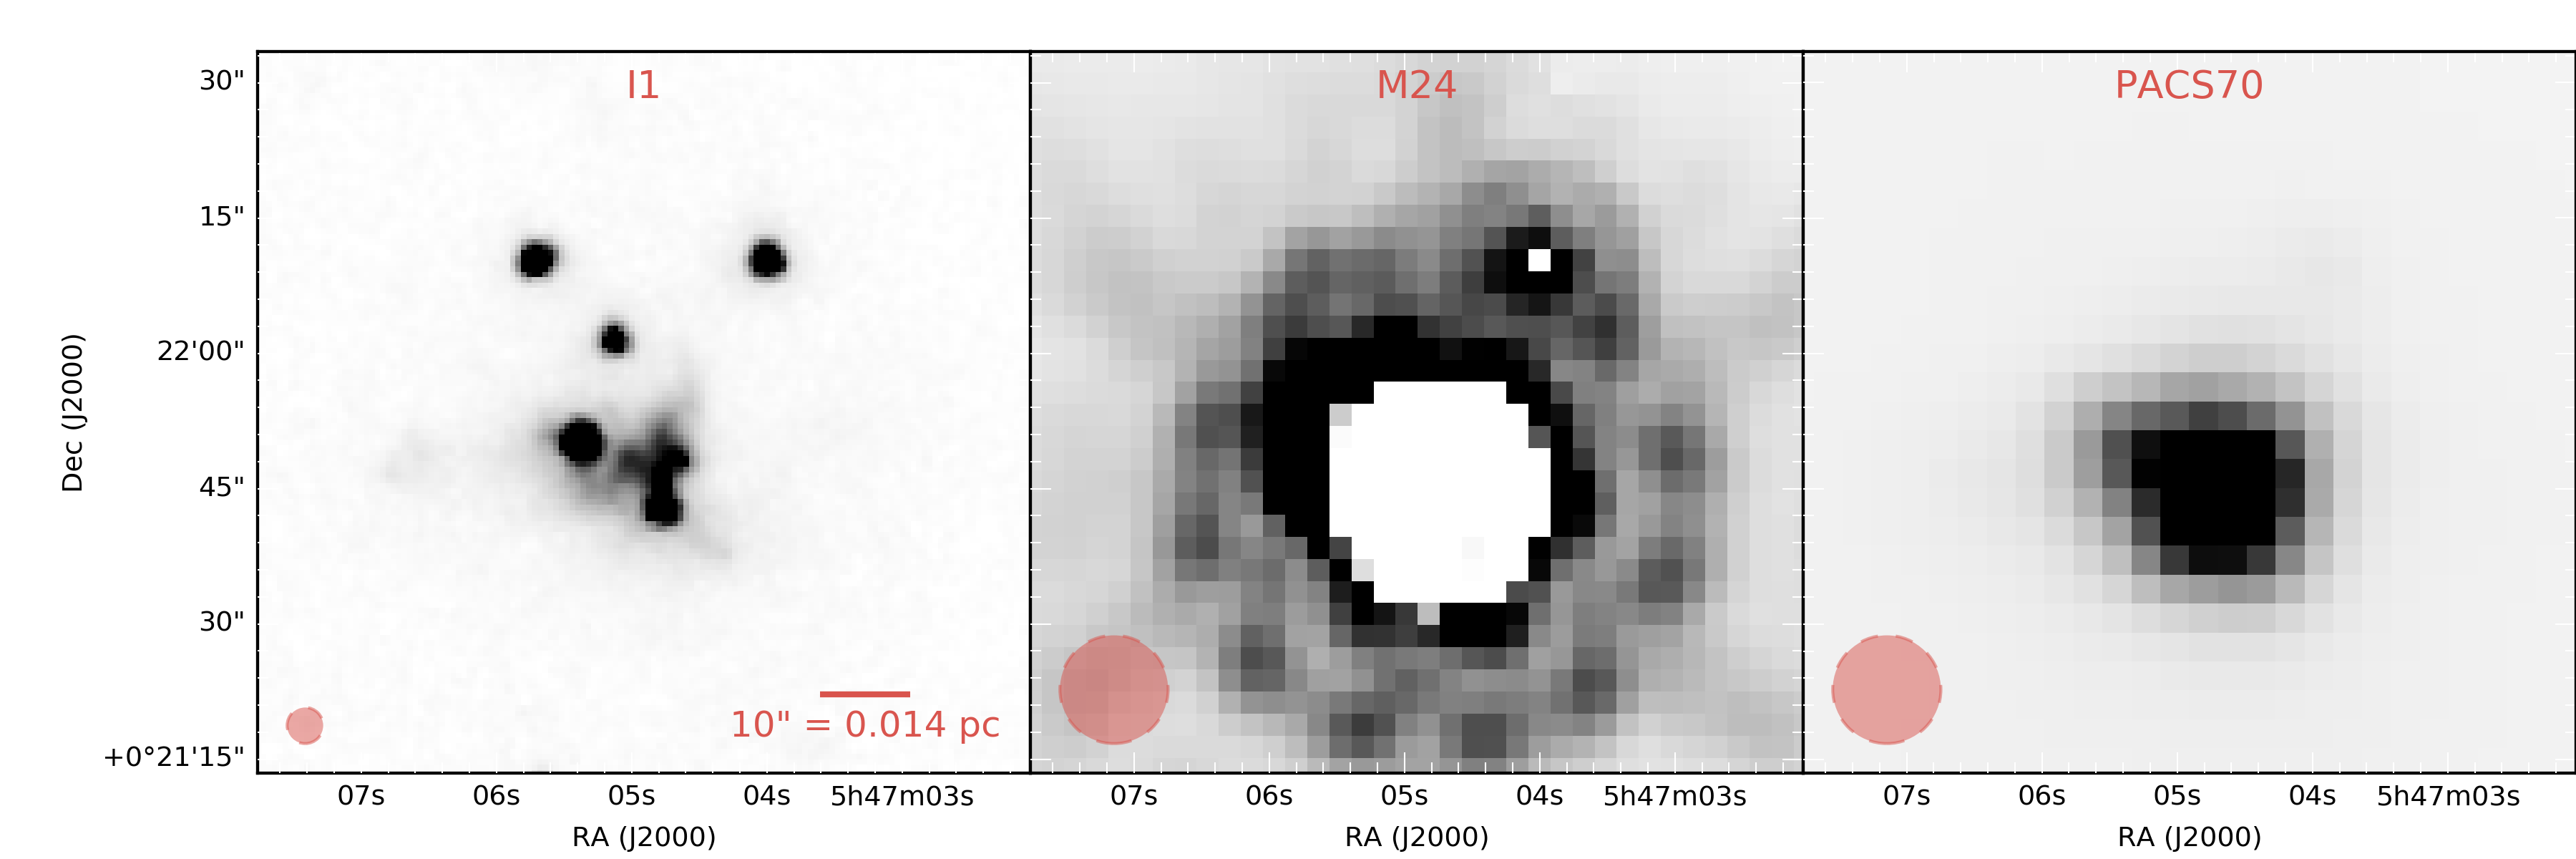
\includegraphics[width=\textwidth]{Figures/NGC2071_saturated_mosaic.png}
\label{fig:NGC20171_saturated}
\caption[Saturation and confusion]{Saturation and confusion in NGC2071.}
\end{center}
\end{figure}

BETTII will tackle the confusion problem at wavelengths from 30 to \SI{100}{\micro\meter}, and will be complementary to \Herschel observations of star-forming regions. SOFIA, however, can already start studying these dense regions with its FORCAST instrument, providing 2-\ang{;;3.5} resolution between 10 and \SI{37}{\micro\meter}. 

We responded to SOFIA FORCAST's first science call with a proposal for a survey of nearby star-forming cluster cores. The clusters were selected from a list of dense young clusters within 1 kpc of the Sun based on \citet{Porras:2003kxa} and \citet{Gutermuth:2009gca}. From this list we selected clusters that were: (1) north of -25 degrees declination so that they could be done from a northern hemisphere flight; (2) included membership of $>$50 YSOs; and (3) included bright 8-\SI{24}{\micro\meter} sources within the dense cores based on \Spitzer and/or WISE data. 

In order to sample the most range of the SED, we proposed to observe in 4 of FORCAST's science continuum bands: 11.1, 19.7, 31.5 and \SI{37.1}{\micron}. This wavelength coverage would be very complementary to archival data from \Spitzer and WISE. Our focus on bright regions spread all across the sky is convenient for SOFIA, and our project would be observed as a gap-filler during the primary science flight legs.

The main objective of the survey is to gather statistics and fill the SED gap between {\Spitzer}'s bands and {\Herschel}'s bands. \Spitzer is often unusable for these targets because of saturation and confusion, and Herschel is confused as well. As it is often the case, \Herschel observations were not available for our targets, making these SOFIA observations the best attempt at observing those regions at mid-IR wavelengths, and our only opportunity to constrain the SED of very clustered YSOs in these regions to infer their physical properties.



Our strategy was successful and we were awarded time during the first and second science cycles of FORCAST (see Tab.~\ref{tab:times}). The data analysis and scientific interpretation is presented in the next few sections. First, we describe our observations, as well as the archival datasets that we use to complement our observations. Second, we properly characterize the systematics of the FORCAST instrument and their variations over multiple science flights spanning multiple years. The data reduction process is then explain, followed by a snapshot of the data products themselves. We then discuss our SED fitting strategy, and fit the SEDs of three of our clusters to derive the physical properties of their embedded YSOs.


\section{Observations}
\label{subsec:SOFIAObservations}

The FORCAST camera has two separate $256\times 256$ pixel infrared arrays that cover the wavelength range from 5.5-\SI{37}{\um} in multiple bands with $\ang{;;0.768}\times\ang{;;0.768}$ pixels. The two arrays can observe simultaneously through a dichroic beam splitter that divides the wavelength range shortward and longward of \SI{26}{\um}. Alternatively, the long wavelength array can be used by itself as the dichroic is removed from the light path, gaining a sensitivity of $\sim 2.5$. We observe the 11.1 and \SI{37.1}{\um} together (hereafter "mode 1") and the 19.7 and \SI{31.5}{\um} together (hereafter "mode 2") . We set the 1$\sigma$ sensitivity threshold to that of a moderately rising SED for a \SI{1.5}{\Lsun} source, which is scaled appropriately for the distance to the cluster. This is an attempt at probing the same luminosities at all distances and obtain a consistent sample of YSOs. 

\renewcommand{\arraystretch}{1.5}
\setlist[itemize,1]{nolistsep,leftmargin=*,labelsep=-\mylen}
\def\labelitemi{--}
\begin{table}[!h]
\scriptsize
\caption{List of desired sensitivities}
\vspace{-0.5cm}
\begin{longtable}{c|cccc|c}
\toprule
Distance & \multicolumn{4}{c|}{1$\sigma$ minimum detectable flux (Jy)} &  Corresponding minimum\\
(pc) & \SI{11}{\um}& \SI{19}{\um}& \SI{31}{\um}& \SI{37}{\um}& \si{\Lsun} \\
\hline
   200.0& 0.1& 0.1& 0.32& 0.7&$\sim$0.5\\
   400.0& 0.1& 0.1& 0.32& 0.6&$\sim$1.5\\
   600.0& 0.05& 0.04& 0.18& 0.25&$\sim$1.5\\
   800.0& 0.02& 0.02& 0.1& 0.12&$\sim$1.5\\
1,000.00& 0.01& 0.01& 0.06& 0.1&$\sim$1.5\\

\bottomrule																																		\end{longtable} 
\caption*{List of desired sensitivities for different distances.}
\label{tab:DesiredSensitivities}
\end{table}



However, for the most nearby clusters, the corresponding observing time was so short that the overhead from the observatory was very costly. Hence, we put a lower threshold to the integration time of \SI{30}{\second}. Similarly, the sensitivity of the \SI{37}{\um} band is such that in order to be consistent with our sensitivity target, this band was heavily driving the  observing time using mode 1. Hence, we observe in this mode as long as is required to meet the sensitivity target for the \SI{11}{\um} band, and request more observations in the \SI{37}{\um} band on its own (hereafter "mode 3"). This allows us to request less total observing time while keeping our sensitivity self-consistent. A summary of our target sensitivities for various distances is shown in Table~\ref{tab:DesiredSensitivities}.

Various observing techniques are available to the FORCAST user to deal with background subtraction. The most robust techniques are very costly in terms of overhead for the observatory, so we decided to be audacious and requested the cheapest observing mode: the Chop-Nod-Chop mode (CNC), combined with 9 ditherings for each field, which dramatically helps when co-adding images together. Most of our data was processed by the SOFIA automated pipeline that provided calibrated Level 2 images, except for the data from the first few flights, for which we received the help of one of FORCAST's Principal Investigator, Dr. Joe Adams, who processed the raw data through his own instrument pipeline.

%\begin{figure}[!h]
%\begin{center}
%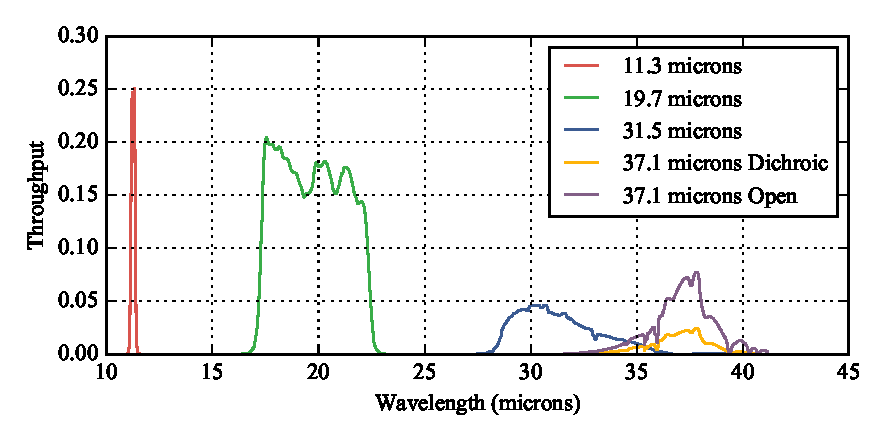
\includegraphics[width=\textwidth]{Figures/SOFIA_bands.pdf}
%\label{fig:SOFIAbands}
%\caption[SOFIA bands]{SOFIA FORCAST bands.}
%\end{center}
%\end{figure}

The data were acquired over 10 SOFIA flights spanning multiple years, with the last batch dating from February 2015. The actual observing times for each band and cluster is shown in Table~\ref{tab:times}. In that table, we have estimated the time for the \SI{37}{\um} band using a composite formula that levels the observing time from mode 3 to that of mode 1, considering their respective sensitivities. We obtained about \SI{10}{\hour} of on-sky data, and 10 out of our 12 original target clusters were observed.

\renewcommand{\arraystretch}{1.5}
\setlist[itemize,1]{nolistsep,leftmargin=*,labelsep=-\mylen}
\def\labelitemi{--}
\begin{table}[!h]
\scriptsize
\caption{List of targets}
\vspace{-0.5cm}
\begin{longtable}{cP{4cm}P{2cm}P{1cm}P{0.5cm}P{0.5cm}P{0.5cm}P{0.5cm}P{0.5cm}}

\toprule																																			
Cluster 	&	 Coordinates 	&	 SOFIA 	&	 $N_\textrm{Fields}$	&	$d $	&	$T_{11} $  	&	$T_{19}  $&	$T_{31}  $&	$T_{37}  $\\
	&	(J2000)	&	Flight IDs	&		&	(pc)	&	(s)	&	(s)	&	(s)	&	(s)	\\
\midrule																	
Cepheus A	&	 22h56m10s +62d03m26s 	&	 F132 F109 	&	2	&	730	&	206	&	234	&	235	&	490	\\
Cepheus C	&	 23h05m45s +62d30m05s 	&	 F132 	&	1	&	730	&	150	&	121	&	121	&	286	\\
IRAS20050	&	 20h07m05s +27d28m51s 	&	 F166 F131 	&	2	&	700	&	321	&	224	&	256	&	266	\\
NGC1333 	&	 03h29m00s +31d17m20s 	&	 F129 F193 F190 	&	9	&	240	&	530	&	558	&	467	&	446	\\
NGC2071 	&	 05h47m06s +00d21m45s 	&	 F192 	&	2	&	420	&	36	&	25	&	33	&	42	\\
NGC2264 	&	 06h41m07s +09d33m35s 	&	 F156 	&	4	&	913	&	495	&	300	&	331	&	587	\\
NGC7129 	&	 21h43m07s +66d06m42s 	&	 F109 	&	1	&	1000	&	383	&	214	&	214	&	709	\\
Ophiuchus 	&	 16h27m05s -24d30m29s 	&	 F157 	&	11	&	150	&	396	&	468	&	501	&	365	\\
S140 	&	 22h19m23s +63d18m44s 	&	 F129 	&	1	&	900	&	322	&	393	&	393	&	568	\\
S171 	&	 00h04m01s +68d34m50s 	&	 F132 	&	1	&	850	&	253	&	219	&	219	&	476	\\\bottomrule																																		\end{longtable} 
\caption*{List of observed targets. For each cluster, we list the SOFIA flights on which the data was taken, the number of individual fields within the cluster, the distance, and the total integration time for each of the 4 observation bands, including all fields. Note that the \SI{37}{\micro\meter} time quote is a composite time calculated by combining the exposure time of mode 1 with that of mode 3, as discussed in the text.}
%List of our 12 proposed targets, with approximate RA and Dec, distance $d$ in parsecs, peak number density in \# stars/pc$^{2}$ from \citep{Gutermuth:2009p1325}, whether the image saturates in Spitzer/in WISE, the number of different fields for each target, the number of YSOs above our threshold level derived from WISE photometry, and the requested time in minutes on source that we request. Note that the latter DOES NOT include overheads.}
\label{tab:times}
\end{table}

To complement our observations, we proceed to an archival search to find publicly available WISE, \Spitzer, and \Herschel images. Most of our targets have already available \Spitzer IRAC and/or MIPS photometry \citep[mostly from][]{Gutermuth:2009gca,Megeath:2012cn,Evans:2009bka}, which we use in the relevant cases. In the cases where no IRAC photometry was available, we applied our own photometry algorithms. We could not find published photometry for the targets with available \Herschel images, hence we also used our own photometry pipeline to derive fluxes. In some cases, we find previously published \SI{1.3}{\milli\meter} continuum measurements to help constrain the long-wavelength behavior of the SEDs.


\section{FORCAST characterization}

In addition to the raw images, a number of calibrators were observed during each flight for different dichroic settings and wavelength bands. These calibrators are usually bright stars which guarantee to be point sources for SOFIA's angular resolution, and have very predictable mid-IR fluxes, so they can be used both for flux and PSF calibration. We use them for two purposes: the first is to obtain a robust metric to determine whether sources are extended or not; the second is to determine the aperture correction factor which will later be used for aperture photometry. 

\subsection{PSF size}
The size of the PSF can be defined in multiple ways, we adopt the approach of characterizing the PSF using its encircled energy distribution. Fig~\ref{fig:average_EE} shows the average of the normalized encircled energy distribution of the PSF, measured on all the calibrators of our sample. Each curve represents one of the five different combinations of bandpass filter and dichroic setting that we use for our observations. For each radius, the total energy is the sum of the pixels within the circular aperture of that radius, to which we subtract an estimate of the background in an annulus around the source (see Section [] for details on the background subtraction methods). 

\begin{figure}[!h]
\begin{center}
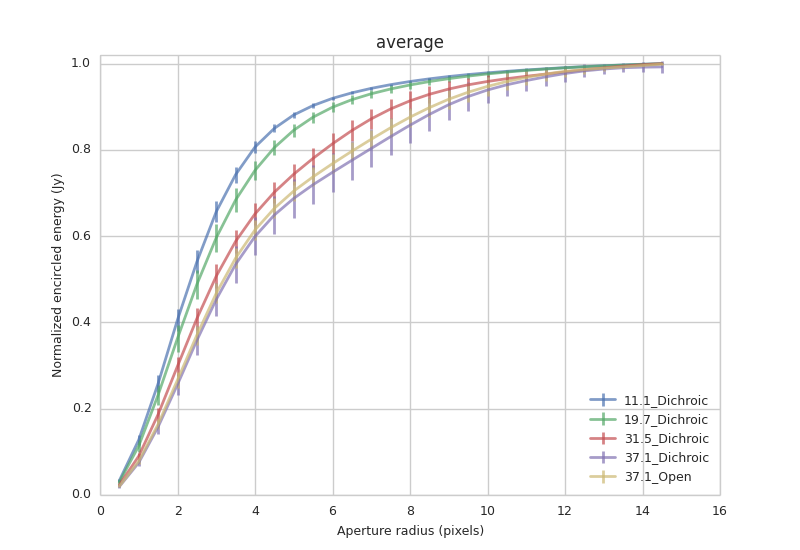
\includegraphics[width=\textwidth]{Figures/average.png}
\label{fig:average_EE}
\vspace{-0.5cm}
\caption[PSF size]{Average PSF encircled energy distribution profile for all calibrator observations.}
\end{center}
\end{figure}


As expected, the PSF at \SI{37.1}{\micro\meter} is larger than the PSFs at shorter wavelengths, but less that the traditional diffraction limit rule. This indicates that additional PSF smearing is occurring at short wavelengths, likely due to plane jitter and pointing errors, which is consistent with what other authors have found \citep[e.g.][]{Herter:2013by}. Throughout all the flights, point source calibrators always have the same encircled energy distribution shape within $\sim~4\%$ rms. 

To look at the behavior of the PSF in more detail, we can use the half width at half maximum of the encircled energy distribution, \Rfifty as a proxy for PSF size. The variation of this quantity for the various flights, bandpass/dichroic setting, and calibrators used is showed in Fig~\ref{fig:Rfifty_dist}. This shows the flight-to-flight differences and, for some calibrators, the in-flight variability. We find that the latter is usually small, except for the SOFIA flight on 05-02-2014, for which the spread is quite considerable and could have been caused by instrumental malfunction or abnormal levels of jitter. The variation from flight to flight is larger than the variation within a given flight, which indicates variability in the observing conditions, systematics, or thermal radiation environment of the observatory between different flights. Even considering the flight-to-flight and calibrator-to-calibrator variations, the overall spread in \Rfifty for a given observation setting is almost always less then 10\%, making this metric a useful reference to compare with scientific data. In our analysis we will compute \Rfifty for our sources and compare it to the \Rfifty from the current flight for the same filter setting, if the calibration file exists. If no calibration file exists for a given setting, we use the mean \Rfifty for that setting from calibrators observations in other flights. The ratio \Rpercent of these two quantities helps quantify the extension of the source, to within $\sim 10\%$. 

\begin{figure}[!h]
\begin{center}
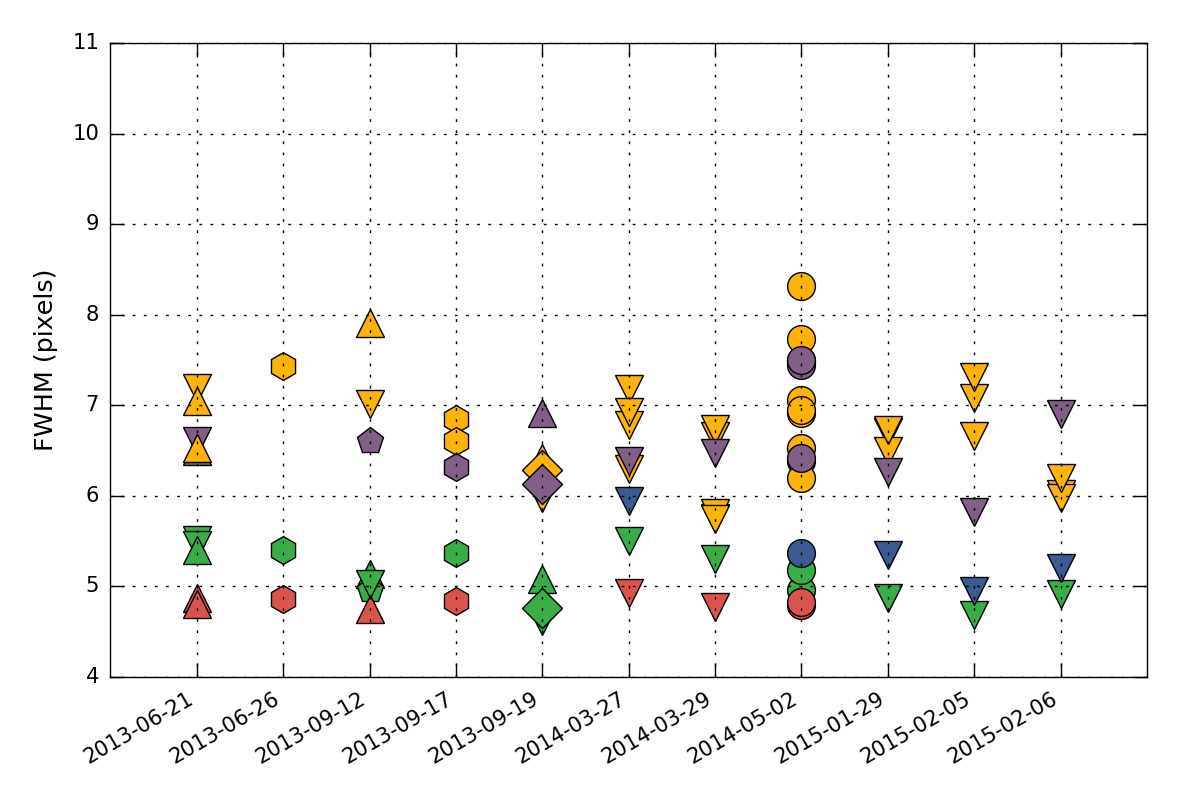
\includegraphics[width=\textwidth]{Figures/R50.png}
\label{fig:Rfifty_dist}
\vspace{-0.5cm}

\caption[PSF size of calibrators]{Distribution of \Rfifty for all calibrators observations within each bandpass. In red: \SI{11}{\um} band, with dichroic; in green: \SI{19}{\um} band, with dichroic; in blue: \SI{31}{\um} band, with dichroic; in yellow: \SI{37}{\um} band, with dichroic; in purple: \SI{19}{\um} band, with dichroic. Down triangles: $\alpha$ Boo; Pentagons: $\alpha$ Cet; Diamonds: $\alpha$ Tau;  Up triangles: $\beta$ And; Hexagons: $\beta$ Peg; Circles: $\beta$ UMi;}
\end{center}
\end{figure}

\subsection{Aperture correction factor}
\label{subsec:apcorr}
In Fig.~\ref{fig:average_EE}, we observe that the encircled energy does not vary much by the time the aperture reaches a radius of 12 pixels, so we consider this fiducial aperture as our "total flux" aperture. The goal of aperture photometry is to estimate the amount of flux in this large aperture, which we consider to be the total amount of flux from the source, by only measuring flux within a much smaller aperture. This has the advantage of reducing contamination from other sources, and increases the signal-to-noise ratio of the flux estimate since the pixels near the tail of the PSF usually contain more noise than signal. 
In Fig~\ref{fig:response}, we plot the aperture correction factor that we compute from the ratio of the flux measured within an aperture of 4 pixels radius and this 12-pixel aperture.  Not surprisingly, this graph follows very closely the plot of $\Rfifty$ from Fig~\ref{fig:Rfifty_dist}, showing the close link between the aperture correction factor and the shape of the calibrator's PSF. We match each observation in our data to the mean of the aperture correction factors for the same observation setting and flight.

\begin{figure}[!h]
\begin{center}
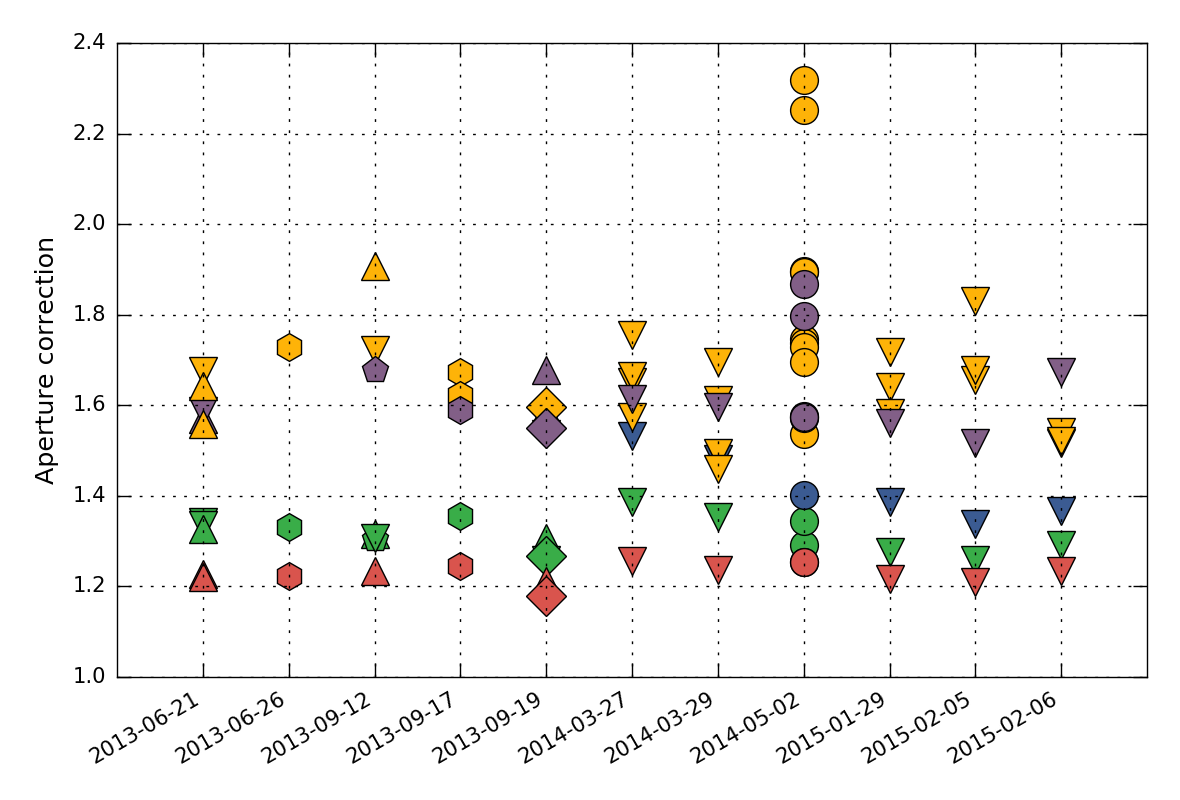
\includegraphics[width=\textwidth]{Figures/Aper_corr.png}
\label{fig:aper_corr}
\vspace{-0.5cm}
\caption[aperture correction]{Instrumental response and aperture correction}
\end{center}
\end{figure}



\subsection{Instrument response and overall uncertainty}
To validate our approach, we take a look at the calibrator fluxes after normalization by the calibration factor, which is provided directly by the FORCAST pipeline. This calibration factors converts the pixel digital value a physical flux density unit, and presumably is determined using the flux from calibrator stars as well. Here we re-measure the flux from each calibrator for each observation setting and each flight, using our standard aperture photometry method and background subtraction. Ideally, we would always obtain the same flux for each setting and calibrator, independently of the flight, an assertion we find true to within $\sim 5\%$. The in-flight errors are typically lower than this. This validates our aperture photometry method, and we can trust that the instrument's systematics are well-behaved to within these levels. 

This would suggest that we can adopt systematic $1\sigma$ uncertainties of $\sim 5\%$, a value which is consistent with the published uncertainties of $3\sigma \approx 20\%$ \citep{DeBuizer:2012ie}.


\begin{figure}[!h]
\begin{center}
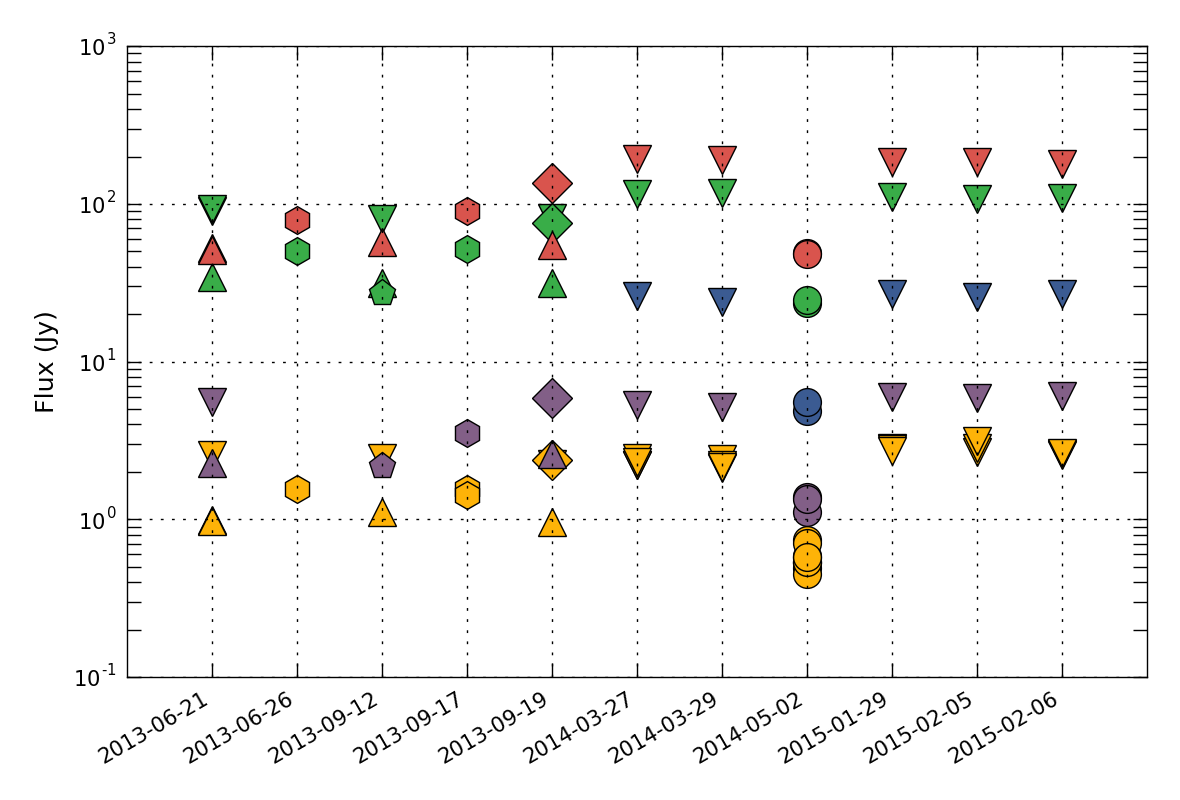
\includegraphics[width=\textwidth]{Figures/Phot_val.png}
\label{fig:response}
\vspace{-0.5cm}
\caption[Instrumental response]{Instrumental response}
\end{center}
\end{figure}




\section{Data reduction and photometry}

The data are processed through various versions of the online pipeline to yield Level 2 data products available on the archive \citep{Herter:2013by}. We apply our own reduction procedure and photometry pipeline on those products to derive final images, source positions, fluxes and sensitivities. Our software makes extensive use of the Python \textit{astropy} package \citep{2013A&A...558A..33A} and its associated modules \textit{photutils} and \textit{APLpy}. 

\subsection{Pre-treatment}
Some manual treatment of each image is necessary before it can be analyzed by our software, which follows this procedure: a) visually aligning the WCS coordinate system, often 10-20" off, using point sources and archival data from other wavelengths and facilities such as IRAC \SI{8}{\micro\meter}; b) cropping the images to clean off the nodded fields, and c) identify the coordinates of each source, both point-like and extended.

After these manual steps, the Level 2 images are multiplied by the calibration factor provided by the online pipeline, which converts them to Jy/pixel. We do not proceed to any systematic color correction, but the effects on the fluxes are very small \citep{Herter:2013by}.
\begin{enumerate}
\item Adjust WCS coordinates: use images at other wavelengths (2MASS, IRAC, MIPS, WISE) to re-align the (RA, DEC) position of the field. We estimate that this process is good to within one SOFIA pixel (\ang{;;0.768}) for the fields where one or more point sources can be identified. Extended fields are less trustworthy, since matching the extended emission to other wavelengths is harder. The rotation of the field produced by the SOFIA pipeline is correct for all of our data. 
\item Crop each image, remove chopped fields, remove artifacts.
\item Identify and categorize sources: isolated point sources, clustered point sources, and extended sources. For extended sources, a circular or elliptical aperture is used to try to encompass the entirety of the emission.
\item Manually identify a location in the field that corresponds to a representative background.
\end{enumerate}

\subsection{Source flux extraction}

We feed the adjusted FITS and associated metadata files to our photometry pipeline. For each identified source, we determine its flux in all bands using aperture photometry with local background subtraction. The aperture correction factor we use is the one determined from the calibrators observed for the same observation setting during this flight. If a calibrator was not available during the flight, we use the average aperture correction factor taken over 9 of our 10 flights (we choose to exclude the flight on 05/02/2014 which seems to have abnormal behavior).

We distinguish between 3 types of sources after manual identification: \textit{isolated}, which are point sources with no nearby objects; \textit{clustered}, which are point sources with nearby objects; and \textit{extended}, which are not consistent with being point sources. 

For point sources that are isolated, we use our standard aperture of 4 pixels at all wavelengths. We consider an annulus surrounding the source extending from 12 to 20 pixels radius (24 to 40 for clustered sources): the local background is determined from the mode of the pixels in the annulus, while the sensitivity is calculated by measuring the standard deviation of the flux values within 4-pixel apertures spread over that annulus [Cite Taro's paper and the Herschel photometry paper that Tracy gave us]. We apply the aperture correction derived from the calibrator observations taken during that flight.

For extended sources, an elliptical aperture is determined manually from the \SI{37}{\micro\meter} images. The local background is determined from the mode of an elliptical annulus, with an inner boundary at the elliptical aperture and an outer boundary corresponding to an ellipse 20\% larger. The sensitivity quoted is the point source sensitivity, and is determined following the same method as for point sources, using the standard deviation of apertures spread across the elliptical annulus. 

The photometry from sources that were observed in different flights is then combined to increase the signal-to-noise ratio. This combination takes into account the sensitivity of each source by appropriately weighing each image.

The source sensitivity calculated is added to the systematic uncertainty of the instrument, for which we follow the recommendation from \citep{Herter:2012hv} to adopt a 7\%, $1\sigma$ uncertainty. 

To validate our flux extraction method, we compare our results with data from \citet{Harvey:2012kw} who observed one of the sources in our sample, S140. Their photometry (shown in their Table 1.) of IRS 1, 2 and 3 (respectively corresponding to our targets S140.5, S140.4, and S140.3) is compared to our photometry in Table~\ref{tab:SOFIAPhotometryHarvey}.

\renewcommand{\arraystretch}{1.5}
\setlist[itemize,1]{nolistsep,leftmargin=*,labelsep=-\mylen}
\def\labelitemi{--}
\begin{table}[!h]
\scriptsize
\caption{SOFIA photometry comparison} \label{tab:SOFIAPhotometryHarvey}
\vspace{-0.5cm}
\begin{longtable}{l|P{1cm}P{1cm}P{1cm}P{1cm}P{1cm}P{1cm}P{1cm}}
\toprule															
SOFIA name	&	F11	&	F11L	&	F19	&	F31	&	F31L	&	F37	&	F37L	\\
\midrule															
S140.3	&	9.79	&	9.7	&	101.70	&	449.60	&	401.00	&	639.17	&	669.00	\\
S140.4	&	3.62	&	4	&	91.09	&	357.63	&	368.00	&	367.35	&	485.00	\\
S140.5	&	110.02	&	110	&	812.84	&	1857.33	&	1585.00	&	2000.94	&	2176.00	\\
\midrule															
Sum of point sources in cluster	&	123.43	&	123.7	&	1005.63	&	2664.57	&	2354	&	3007.47	&	3330	\\
Total cluster emission	&	135.26	&	145	&	1195.20	&	4450.31	&	3780.00	&	5910.26	&	6730.00	\\
Error (\%)	&	9.59	&	17.22	&	18.85	&	67.02	&	60.58	&	96.52	&	102.10	\\
\bottomrule					
	\end{longtable} 
\caption*{Comparison of SOFIA four-band photometry from \citet{Harvey:2012kw} on S140 (columns with 'L'). The authors' "total emission" actually represents the total emission in the entire field of view, whereas out measurement corresponds to a manually-selected source region encompassing only the dense core. The total emission in the entire field of view is less representative, as it could include contribution from other sources as well as areas of negative flux from the chopping and nodding steps. In this cluster, there is a large amount of emission which is not due to the three identified sources.}

\end{table}

\subsection{Image sensitivity}
In order to determine the absolute sensitivity in the image, we use two methods. First, we manually determine a region in each cluster that visually appears devoid of flux. We calculate the sensitivity as if this background region was a source, by patching apertures in an annulus around this background location and calculating the standard deviation of the obtained fluxes. We call this sensitivity measurement $\sigman$. The main downside of this method is that it requires a manual operation to select the appropriate background field, and hence could have more variation depending on which field we select. Second, we use a routine that iteratively isolates the pixel values above $2\sigma$ of the image, in order to remove the contamination from our actual sources. The standard deviation of the resulting image is then calculated, and is multiplied by the square root of the number of pixels in an aperture of 4 pixel radius. This corresponds to a floor sensitivity $\sigstd$. We present our results in Table~\ref{tab:SOFIASensitivity}, where we also compare this sensitivity with the expected sensitivity $\sigth$ obtained using the online calculator with the actual exposure time of our images. We note that usually, the theoretical values are more in agreement with our first method. 

\renewcommand{\arraystretch}{1.5}
\setlist[itemize,1]{nolistsep,leftmargin=*,labelsep=-\mylen}
\def\labelitemi{--}
\begin{table}[!h]
\scriptsize
\caption{FORCAST Sensitivities}
\vspace{-0.5cm}
\begin{longtable}{c|P{0.5cm}P{0.5cm}P{0.5cm}|P{0.5cm}P{0.5cm}P{0.5cm}|P{0.5cm}P{0.5cm}P{0.5cm}|P{0.5cm}P{0.5cm}P{0.5cm}|P{1cm}}
\toprule																			
Cluster 	&	\multicolumn{3}{c|}{F11}					&	\multicolumn{3}{c|}{F19}					&	\multicolumn{3}{c|}{F31}					&	\multicolumn{3}{c|}{F37}					&	 Sources 	\\
	&	$\sigman$ 	&	$\sigstd$ 	&	$\sigth$	&	$\sigman$ 	&	$\sigstd$ 	&	$\sigth$	&	$\sigman$ 	&	$\sigstd$ 	&	$\sigth$	&	$\sigman$ 	&	$\sigstd$ 	&	$\sigth$	&		\\
\midrule																											
CepA 	&	0.07	&	0.04	&	0.05	&	0.11	&	0.05	&	0.05	&	0.19	&	0.07	&	0.16	&	0.26	&	0.09	&	0.34	&	4	\\
CepC 	&	0.03	&	0.03	&	0.04	&	0.10	&	0.05	&	0.04	&	0.19	&	0.06	&	0.16	&	0.16	&	0.09	&	0.30	&	4	\\
IRAS20050 	&	0.04	&	0.03	&	0.04	&	0.08	&	0.04	&	0.05	&	0.13	&	0.05	&	0.16	&	0.30	&	0.11	&	0.32	&	7	\\
NGC1333 	&	0.12	&	0.04	&	0.07	&	0.07	&	0.07	&	0.07	&	0.22	&	0.08	&	0.25	&	0.48	&	0.13	&	0.52	&	11	\\
NGC2071 	&	0.19	&	0.10	&	0.12	&	0.32	&	0.15	&	0.15	&	0.21	&	0.22	&	0.49	&	0.45	&	0.28	&	0.81	&	6	\\
NGC2264 	&	0.07	&	0.03	&	0.05	&	0.19	&	0.05	&	0.06	&	0.28	&	0.07	&	0.20	&	0.21	&	0.09	&	0.43	&	21	\\
NGC7129 	&	0.07	&	0.03	&	0.03	&	0.10	&	0.04	&	0.03	&	0.26	&	0.09	&	0.12	&	0.17	&	0.08	&	0.19	&	5	\\
Ophiuchus 	&	0.11	&	0.05	&	0.08	&	0.16	&	0.07	&	0.08	&	0.31	&	0.09	&	0.27	&	0.41	&	0.18	&	0.65	&	19	\\
S140 	&	0.04	&	0.03	&	0.03	&	0.16	&	0.03	&	0.03	&	0.21	&	0.07	&	0.09	&	0.35	&	0.11	&	0.21	&	7	\\
S171 	&	0.04	&	0.03	&	0.03	&	0.07	&	0.04	&	0.03	&	0.07	&	0.05	&	0.12	&	0.16	&	0.06	&	0.23	&	2	\\
\bottomrule					
	\end{longtable} 
\caption*{For each band, we measure the 1$\sigma$ sensitivity \sigman and \sigstd in each field from the data using two different methods (see Section~\ref{} for details), and present here the median of all fields. The theoretical sensitivity \sigth corresponds to the expected sensitivity for the effective integration time, using the SOFIA FORCAST observation planning tools. All sensitivity values are in Janskies.}
%List of our 12 proposed targets, with approximate RA and Dec, distance $d$ in parsecs, peak number density in \# stars/pc$^{2}$ from \citep{Gutermuth:2009p1325}, whether the image saturates in Spitzer/in WISE, the number of different fields for each target, the number of YSOs above our threshold level derived from WISE photometry, and the requested time in minutes on source that we request. Note that the latter DOES NOT include overheads.}
\label{tab:SOFIASensitivity}
\end{table}


\subsection{Other photometry}

While SOFIA provides mid-IR photometry, we looked in the literature for published fluxes on our targets in order to reconstruct more complete SEDs. In addition to our four SOFIA bands, our table includes data from 2MASS, \Spitzer, and other instruments. Photometry from these sources is published in online catalogs, which we programmatically cross-reference with the positions of our targets. The closest target that corresponds to a Vizier location query is selected to be the correct catalog match. For the 2MASS data, the location of the target needs to be less than \ang{;;2} away from our coordinates for point sources, and \ang{;;5} for extended sources. For the \Spitzer data, the matching radius is \ang{;;3} for point sources and \ang{;;10} for extended sources. In addition to automated online catalog searches, we also add values for sources in NGC2071 from \citet{vanKempen:2012fb}.

For our two most clustered cases in the cores of NGC2071 and IRAS20050+2720, the published catalogs do not have all available fluxes. We assume that the sources are so clustered that they the source extraction software from these authors do not register them as point sources, due to confusion or saturation effects. Hence we adapt our own photometry routines for these clustered environments and obtain the fluxes directly from the calibrated Level 3 images themselves, which are all available on the archive. In Table~\ref{tab:SpitzerPhotometry}, we compare our photometry results with published fluxes from \citet{Megeath:2012cn} and \citet{Gutermuth:2009gca} for isolated sources elsewhere in these same fields of view. We use the \Spitzer handbook recommendations for aperture photometry on \Spitzer archival images (\ang{;;2.4} aperture with and an annulus that extends from 12 to \ang{;;20}). We find that our results are within 10\% of these other authors' results, although it is possible that we are systematically overestimating the fluxes. 

\renewcommand{\arraystretch}{1.5}
\setlist[itemize,1]{nolistsep,leftmargin=*,labelsep=-\mylen}
\def\labelitemi{--}
\begin{table}[!h]
\scriptsize
\caption{Spitzer photometry comparison}
\vspace{-0.5cm}
\begin{longtable}{l|P{1cm}P{1cm}P{1cm}P{1cm}}
\toprule																			
SOFIA name	&	i1	&	i2	&	i3	&	i4	\\
\midrule									
NGC2071.1	&	0.04	&	0.06	&	0.02	&	-0.03	\\
NGC2071.3	&	-0.07	&	-0.10	&	-0.06	&	-0.09	\\
NGC2071.4	&	0.04	&	-0.12	&	-0.01	&	-0.10	\\
NGC2071.5	&	-0.05	&	-0.06	&	-0.11	&	-0.11	\\
\midrule									
IRAS20050.1	&	-0.08	&	-0.06	&	-0.07	&	0.08	\\
IRAS20050.3	&	0.19	&	0.10	&	0.05	&	0.10	\\
IRAS20050.6	&	-0.07	&	-0.06	&	-0.12	&	-0.05	\\
IRAS20050.7	&	-0.15	&	-0.07	&	-0.02	&	-0.07	\\
\bottomrule					
	\end{longtable} 
\caption*{Fractional difference between our own aperture photometry on \Spitzer archival images and published \Spitzer photometry from \citet{Megeath:2012cn} for NGC2071, and \citet{Gutermuth:2009gca} for IRAS20050+2720. When values are negative, it means that their photometry is lower than ours.}
\label{tab:SpitzerPhotometry}
\end{table}

In some cases, we also found archival Herschel images, although no published photometry was available for most our sources. We then apply our same aperture photometry routines for those calibrated Herschel images, using aperture and background subtraction parameters from \citep{Shimizu:2016if} for the PACS and SPIRE. Because of the very large beams of Herschel compared to FORCAST, the SPIRE bands are considered upper limit fluxes for sources that are further than \SI{300}{\pc}.

\section{Data products}

\subsection{Maps}

The SOFIA FORCAST archival images consist of $\sim~200$ individual images, each representing a field at a given wavelength. Some fields are revisited multiple times when the entire observation could not happen in a single flight leg. These individual fields are processed and mosaiced together to form one single map for each wavelength and each cluster. 

Before mosaicing the fields, we proceed to a 2D background subtraction. This method divides the images into sections of $50\times 50$ pixels, estimates the median in each cell, and fits a 2D function to these median values. This function is then used to construct a smooth background, which is then completely removed from the image. Each background-subtracted image is then calibrated (using the calibration factor that is supplied by the FORCAST pipeline), and weighed by its exposure time before it is co-added into a mosaic in the WCS coordinate frame. Note that although these maps are useful to take a quick glance at the flux distribution and spot artifacts, the actual photometry described in the previous sections uses each individual raw field, without background subtraction. If a source is present in multiple fields, the photometry from each of these fields is combined to provide a better flux estimate.

In Fig.~\ref{fig:variety_sources} we present a variety of maps from our cluster sample. Each map is a three-color image (red: \SI{37}{\micron}, green: \SI{31}{\micron} and blue: \SI{19}{\micron}), and the scale and stretch of each color is adjusted to balance each color. 

\begin{figure}[!h]
\begin{center}
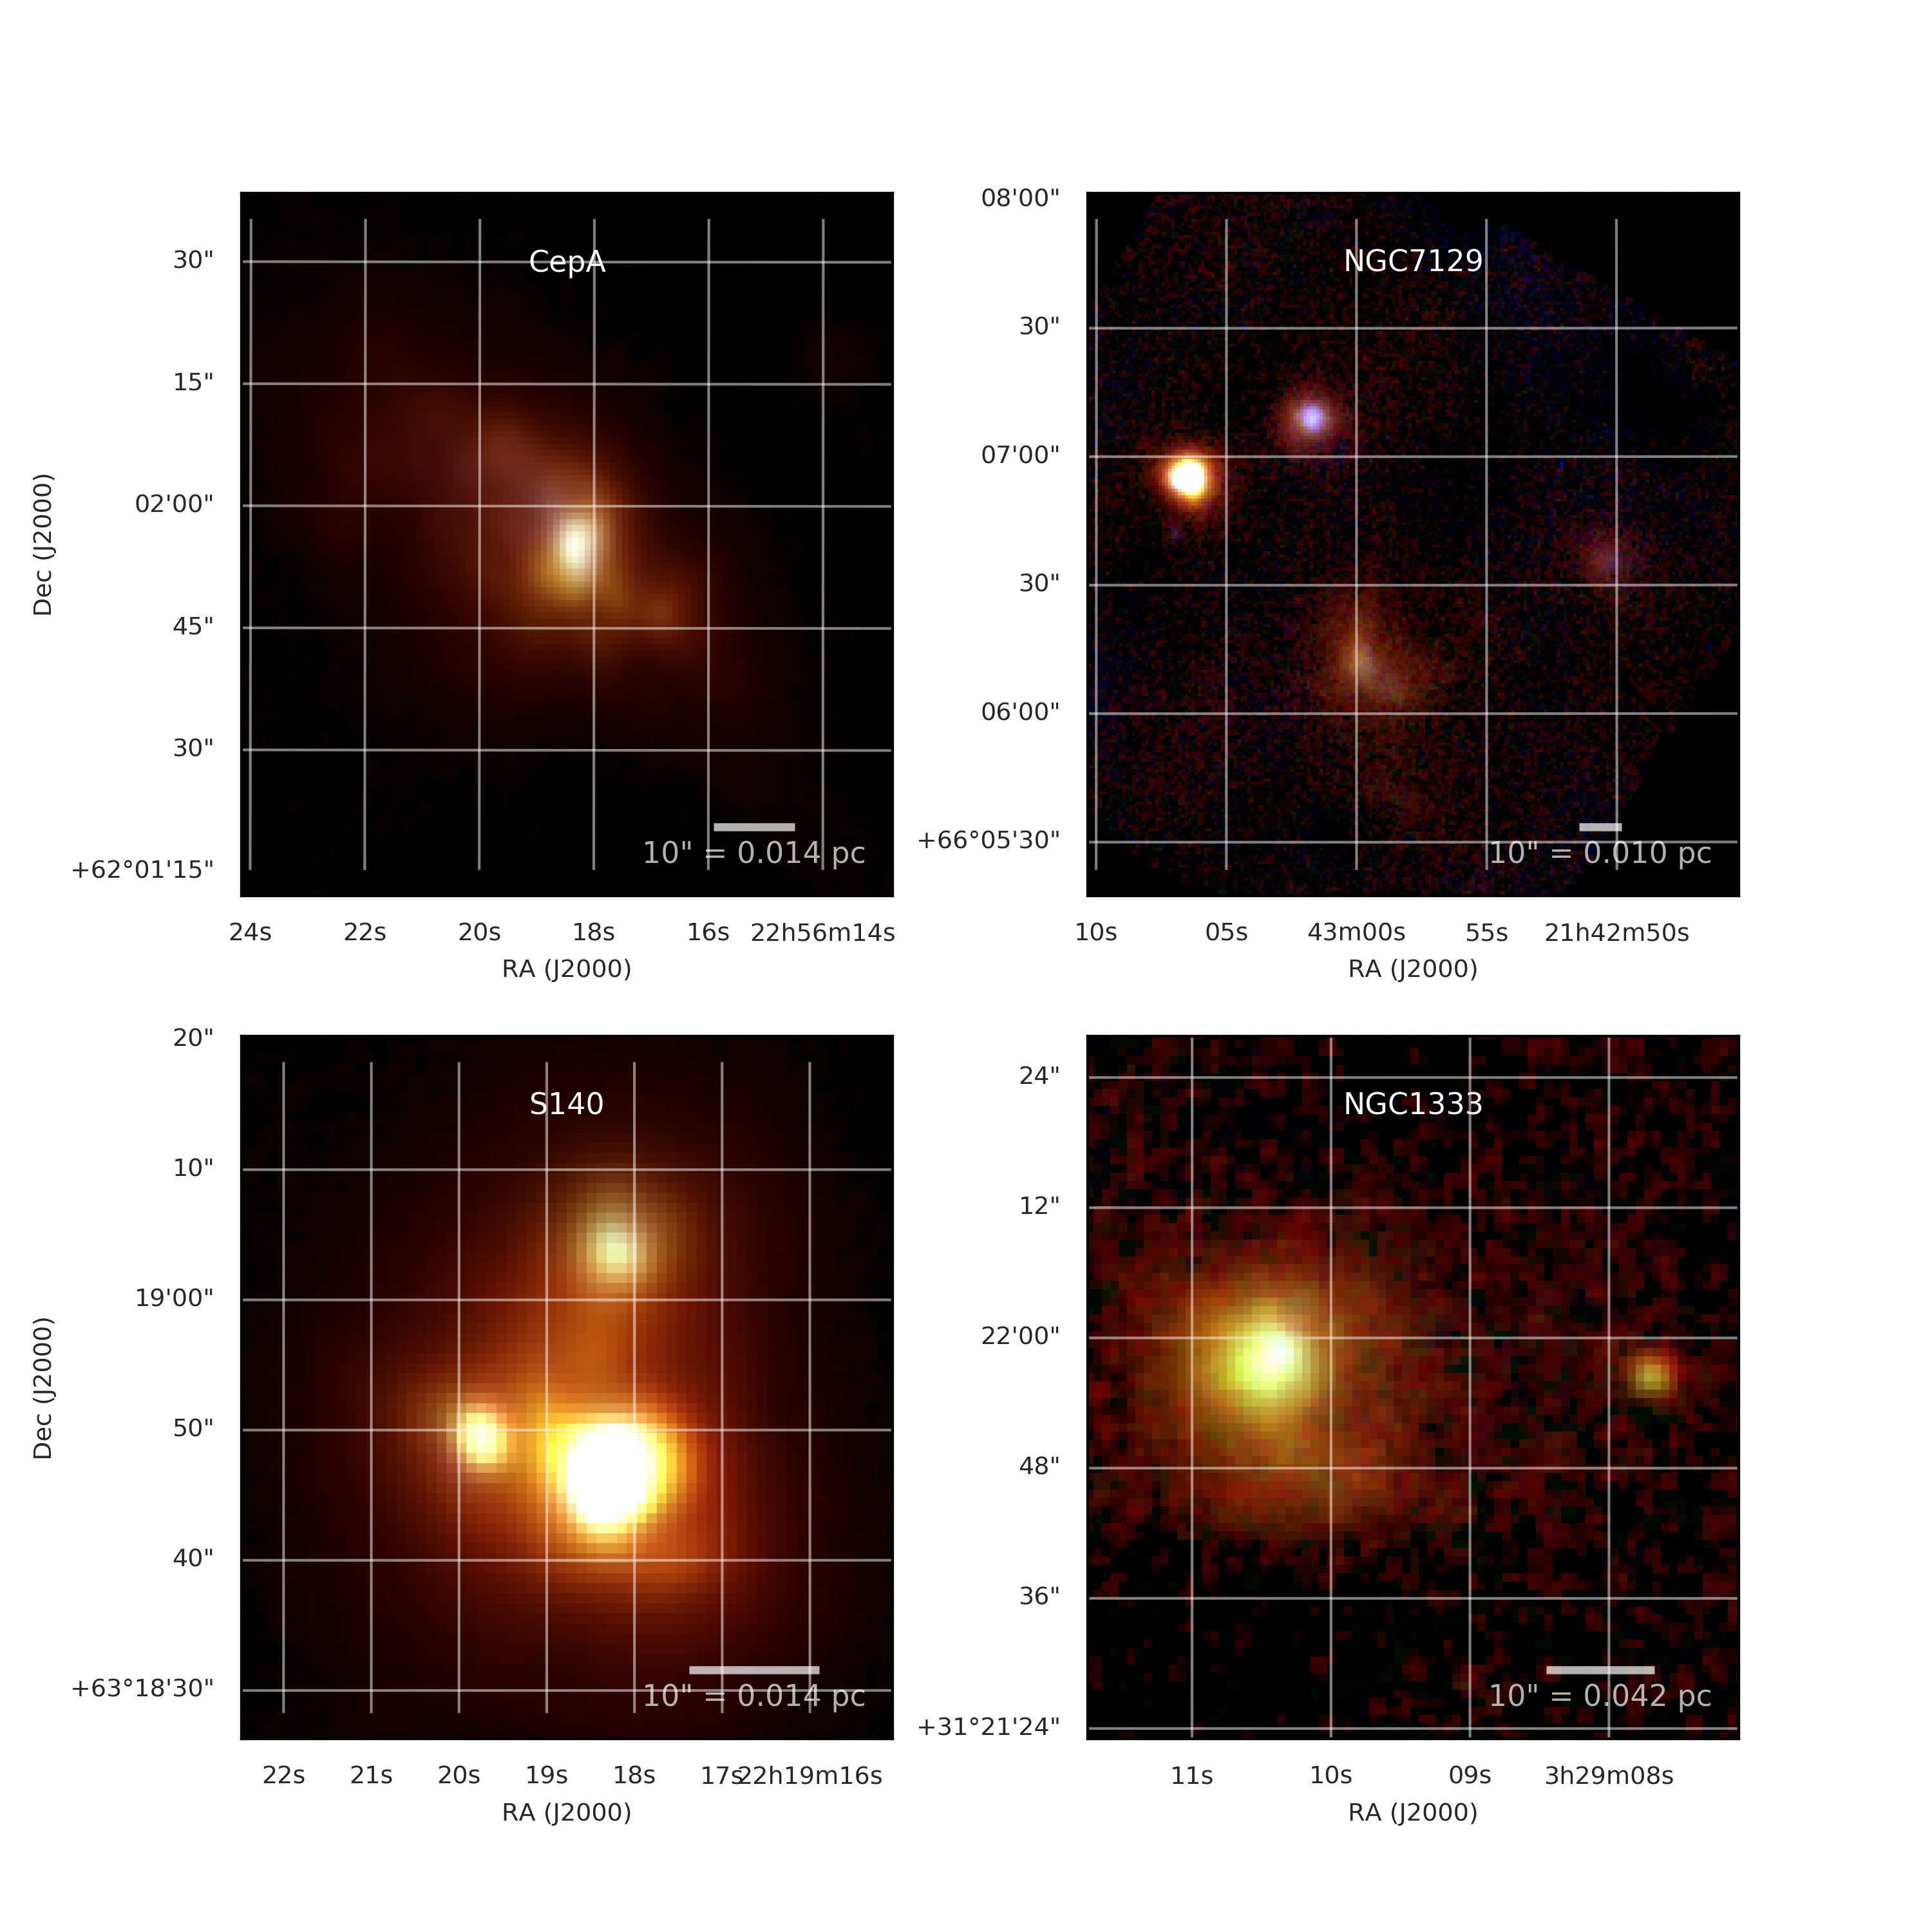
\includegraphics[width=\textwidth]{Figures/RGBmosaic.png}
\label{fig:variety_sources}
\vspace{-1cm}
\caption[RGB images of select sample of sources]{Selected sample of sources}
\end{center}
\end{figure}


\subsection{Source types}
The point sources in our sample are almost exclusively class 0 and I protostars, using the traditional spectral index determination (which uses wavelengths from \SI{2}{\micron} to \SI{24}{\micron}. They all have a spectral index from 0 to 0.2, which indicates the rising SED of an embedded object. However, for a large fraction of our sample, \Spitzer \SI{24}{\um} is unavailable, which makes the spectral index rely only on the 2-\SI{8}{\um} flux to determine the stage of the object. 

We suggest using SOFIA's bands for a more robust estimate of the spectral index. Using wavelengths from 2 to \SI{37}{\um} gives more leverage and avoids misidentification. The difference in the distributions is show in Fig.~\ref{fig:SpectralIndex}.
\begin{figure}[!h]
\begin{center}
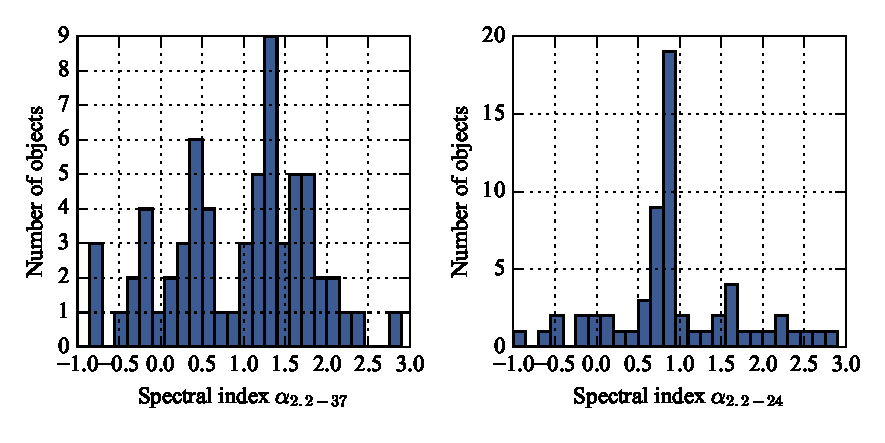
\includegraphics[width=\textwidth]{Figures/SpectralIndex.pdf}
\label{fig:SpectralIndex}
\vspace{-1cm}
\caption[Spectral Index distribution of point sources]{Spectral Index distribution of point sources. \textit{Left}: standard determination of the spectral index, using 2MASS and \Spitzer from \SI{2}{\micron} to \SI{24}{\micron}, when data is available. \textit{Right}: Determination of the spectral index using data from 2MASS, \Spitzer and our FORCAST data up to \SI{37}{\micron}. The distribution changes significantly when you account for the longer fluxes in these clustered regions.}
\end{center}
\end{figure}


\section{SED fitting}

\subsection{A small grid of models}

SED fitting is prone to many degeneracies: usually many geometrical and physical parameters are used to construct detailed radiative transfer models, but only a handful of measurement points are available to fit, leading to a dramatically under-constrained problem. As our starting point of our investigation of the SEDs of these sources, we used the \textit{sedfitter} tool from \citep{Robitaille:2006cb}. These authors computed a large grid of tens of thousands of SED models using a radiative transfer code by \citep{Whitney:2003ke}, by varying 14 geometrical and physical parameters in the dust density grid such as the size of the disk, the accretion rates, the radius and mass of the envelope, etc. The models are then evaluated in the bands corresponding to our data, and a $\chi^2$ metric is evaluated for each model. By exploring the distribution of $\chi^2$, we noticed, as expected, the very large correlations between the parameters which is indicative of many local minimas in the grid. Hence, inferring geometrical and physical parameters from such a grid can be misleading.

We used a more modern version of the same core radiative transfer code, called Hyperion, to develop our own capability of simulating SEDs and understand the sensitivity of these parameters on the SED shape of our Class 0 and I sources. Based on our investigation, the degeneracy between viewing angle and multiple geometrical parameters is considerable. In particular, the sensitivity of the disk properties is minimal, as most of the SED properties are determined almost entirely by the envelope. In addition, parameters of the central source such as the mass, radius and temperature are irrelevant, as they are all combined into one single term, which is the central luminosity. Similarly, the luminosity created when simulating a disk accreting onto the central object can not be distinguished from a more luminous central object and a non-accreting disk. Finally, we find that there is very little difference between Ulrich envelope models and standard power-law envelopes (see for example Fig.~14 from \citet{Whitney:2013cw}), except that the latter can more directly be related to physical parameters such as the mass. 

From these findings, we created a simplified grid of models by significantly reducing the number of parameters. The resulting choices are presented in table []. Note that unlike most authors, who use multiple kinds of dust models for different regions of the SED (which add complexity and number of parameters), we simply use the same dust model for both the envelope and the disk: OH5. 


\renewcommand{\arraystretch}{1.5}
\setlist[itemize,1]{nolistsep,leftmargin=*,labelsep=-\mylen}
\def\labelitemi{--}
\begin{table}[!h]
\scriptsize
\caption[SED model grid]{SED model grid.}
\label{tab:SEDModelGrid}
\vspace{-0.5cm}
\begin{longtable}{lP{5cm}P{3cm}P{2cm}}
\toprule																			
Parameter	&	Description	&	Values	&	Units	\\
\midrule							
\midrule							
\multicolumn{4}{c}{Constant parameters}							\\
\midrule							
\multicolumn{4}{c}{Central source}							\\
\Mstar	&	Stellar mass	&	1	&	\si{\Msun}	\\
\Tstar	&	Stellar temperature	&	4000	&	K	\\
\midrule							
\multicolumn{4}{c}{Disk}							\\
Type	&	Flared or alpha disk	&	Flared	&		\\
\Mdisk	&	Disk mass	&	0.01	&	\si{\Msun}	\\
\Rdiskmax	&	Disk outer radius	&	100	&	\si{\au}	\\
\Rdiskmin	&	Disk inner radius	&	 sublimation radius	&	\si{\au}	\\
$\beta$	&	Flaring parameter	&	1.25	&		\\
$p$	&	Disk surface density exponent	&	-1	&		\\
$r_0$	&	Reference distance for scale height	&	\Rdiskmin	&	\si{\au}	\\
$h_0$	&	Disk scale height at $r_0$	&	0.01\Rdiskmin	&	\si{\au}	\\
$d$	&	Dust	&	OH5	&		\\
\midrule							
\multicolumn{4}{c}{Envelope}							\\
Type	&	Power-law or Ulrich	&	Power-law	&		\\
\Renvmin	&	Envelope inner radius	&	\Rdiskmin	&	\si{\au}	\\
\Renvmax	&	Envelope outer radius	&	5000	&	\si{\au}	\\
$\alpha$	&	Power	&	-1.5	&		\\
$r^\textrm{env}_0$	&	Reference radius	&	\Renvmin	&	\si{\au}	\\
$d$	&	Dust	&	OH5	&		\\
\midrule							
\multicolumn{4}{c}{Cavity}							\\
$r^\textrm{cav}_0$	&	Cavity outer radius	& 	\Renvmax	&	\si{\au}	\\
$\theta_0$	&	Opening angle at $r^\textrm{cav}_0$	&	10	&	degrees	\\
	&	Flaring exponent	&	1.5	&		\\
$\rho_0$	&	Density at $r^\textrm{cav}_0$	&	0	&	\si{\gram\per\centi\meter}	\\
$\alpha_e$	&	Density profile exponent	&	0	&		\\
\midrule							
\midrule							
\multicolumn{4}{c}{Changing parameters}							\\
\midrule							
$i$	&	Inclination angle	&	0 to 90 in 20 constant increments of cos(i)	&	degrees	\\
\Lstar	&	Central luminosity	&	$5\times 1.5^p$ for $p=-4, -3, \dots 15$ (from 0.99 to 288)	&	\si{\Lsun}	\\
\Menv	&	Envelope mass	&	$0.01\times 1.5^p$ for $p=-2, -1, \dots 20$ (from 0.004 to 22.17)	&	\si{\Msun}	\\
\Av	&	External extinction	&	$0, 1, \dots 15$	&		\\
$s$	&	Scaling	&	0.7, 0.85, 1, 1.5, 1.3	&		\\
\bottomrule					
	\end{longtable} 
\end{table}

The parameters in this grid correspond to those used by the Hyperion software. We constructed a wrapper program that can run the Hyperion software for the parameters in this grid. Because of time and resource limitations, a moderate number of photons was chosen. The details of our modeling parameters, which will be familiar to the Hyperion user, are described in Table~\ref{tab:HyperionParams}.

\renewcommand{\arraystretch}{1.5}
\setlist[itemize,1]{nolistsep,leftmargin=*,labelsep=-\mylen}
\def\labelitemi{--}
\begin{table}[!h]
\scriptsize
\caption[Hyperion simulation parameters]{Hyperion simulation parameters.}
\label{tab:HyperionParams}
\vspace{-0.5cm}
\begin{longtable}{lP{4cm}}
\toprule																			
Number of photons (initial)	&	\num{2e5}	\\
Number of photons (imaging)	&	\num{2e5}	\\
Number of photons (raytracing sources)	&	\num{1e6}	\\
Number of photons (raytracing dust)	&	\num{1e6}	\\
Lucy max iterations	&	6	\\
Max photon interactions	&	\num{1e5}	\\
Geometrical grid parameters (radial, theta and azimuthal)	&	400, 199, 2	\\
MRW	&	TRUE	\\
\bottomrule					
	\end{longtable} 
\end{table}

\section{Application to four clusters}

\subsection{IRAS20050+2720}

IRAS~20050+2720 is part of an active site of intermediate-mass star formation in the Cygnus Rift located at 700~pc \citep{Wilking:1989el}, with the particularity that it doesn't seem to contain any massive stars \citep{Gunther:2012dq}. The main cluster core is associated with water and methanol masers \citep{Palla:1991up,Fontani:2010cf} and multipolar molecular outflows observed at millimeter wavelengths \citep{Bachiller:1995cy,Anglada:1998uu,Beltran:2008gu}, suggesting that the region might have experienced a recent episode of star formation in the past 0.1 Myr which contrasts with the average age of the cluster of 1 Myr \citep{Chen:1997tb,Gutermuth:2005hx}. \cite{Gutermuth:2009gca} have identified $>170$ YSOs surrounding the core and measured their continuum fluxes up to \SI{8}{\micro\meter} with IRAC. While measurements at longer wavelengths were able to provide estimates of the total mass of the cluster \citep[e.g. using IRAS,][\SI{388}{\Lsun}]{Molinari:1996td}, the measurements are confused in the densest region and it has not been possible to properly associate the far-IR emission with its short wavelength counterpart because of the small separation between IRAC-detected protostars. The IRAS point source was classified as a luminous class 0 protostar \citep{Bachiller:1996ja}, and its emission associated with the bright millimeter source MMS1 to the northwest of the core \citep{Chini:2001fa}. \cite{Beltran:2008gu} show strong evidence that this region has multiple generations of stars, and suggest that a group of low-mass stars first completed its main accretion phase, before setting the stage for the birth of new intermediate-mass stars at the core of this cluster.

We have observed two fields within the cluster (see Fig.~\ref{fig:IRAS20050_RGB}), including the brightest core at $20^h 07^m 06.70^s +\ang{27;28;54.5}$. Multiple sources in the core can be distinguished in the IRAC maps, but the core appears extended in \Spitzer MIPS at \SI{24}{\micro\meter}, and is identified as a single source with WISE. No good high resolution far-infrared continuum data longward of \SI{24}{\micro\meter} was available for this source.

\begin{landscape}
\begin{figure}
\begin{center}
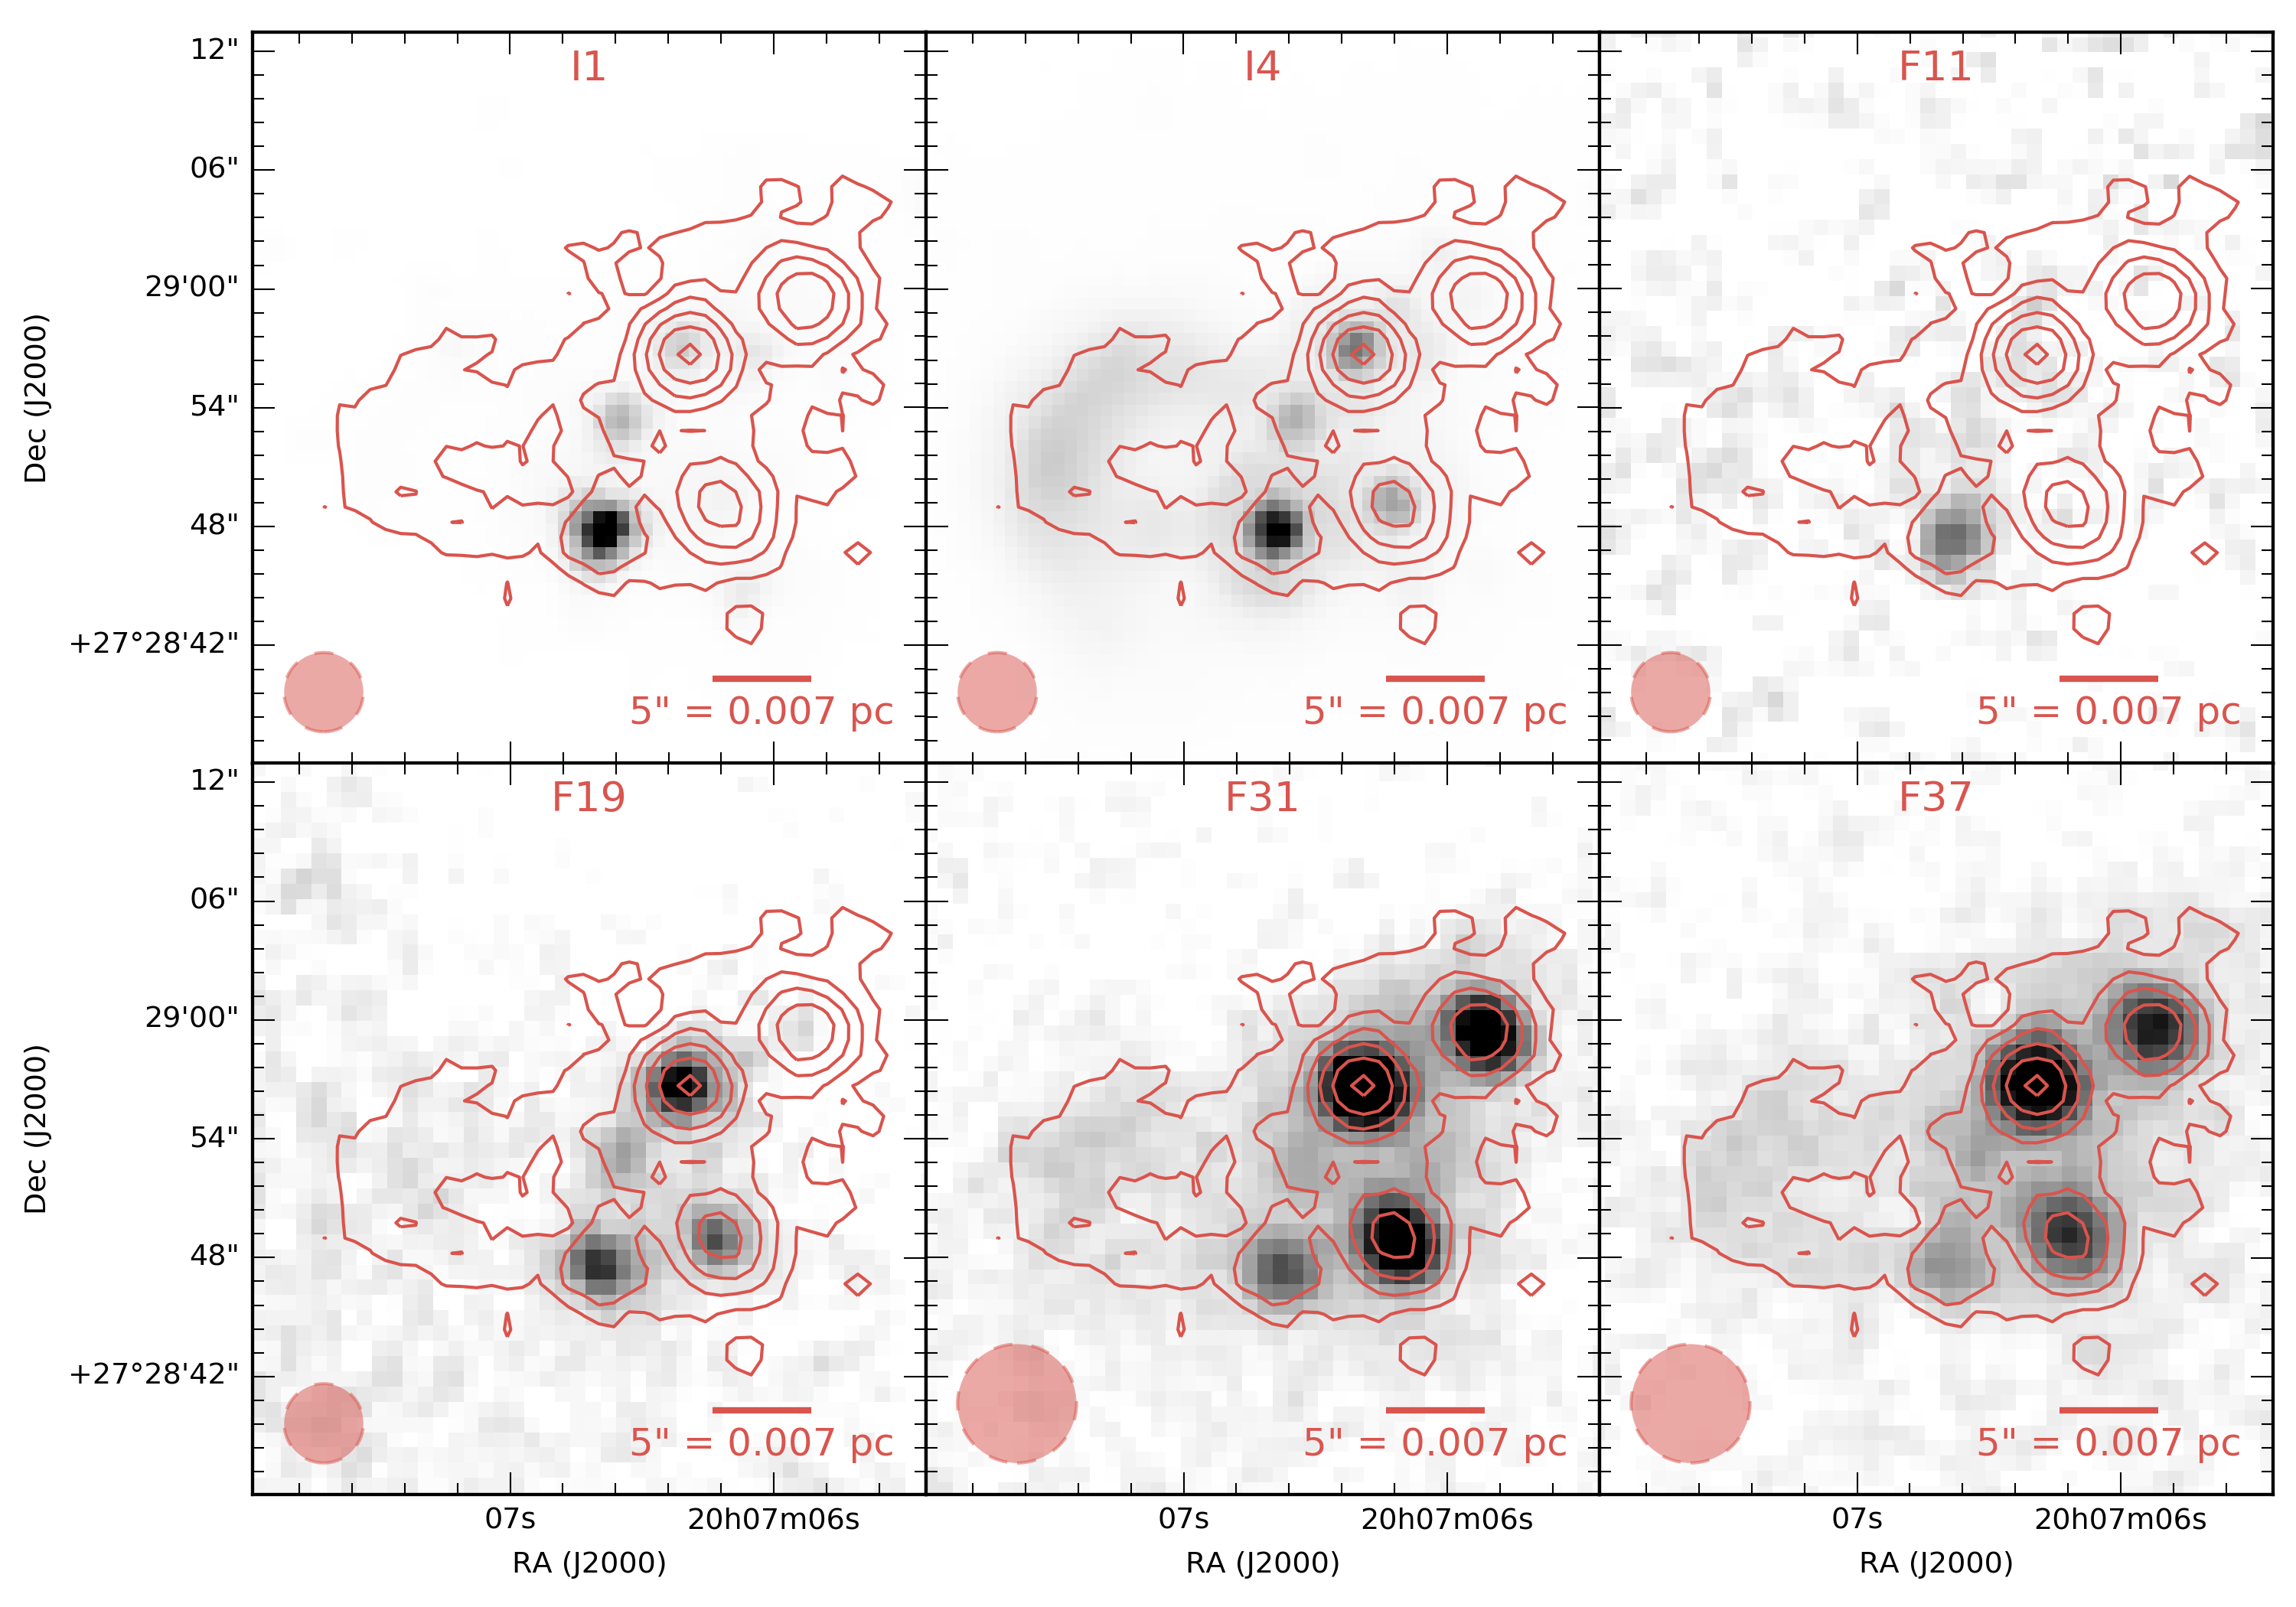
\includegraphics[width=1.5\textwidth]{Figures/IRAS20050.png}
\label{fig:IRAS20050_mosaic}
\vspace{-1cm}
\caption{The core of IRAS20050+2720 is seen in the four bands of the \textit{Spitzer} IRAS instrument, as well as with the four FORCAST bands. The increased resolution of FORCAST compared to previous instruments allows to match the long-wavelength emission with its short wavelength counterpart. The stretch in each image is adjusted for optimal readability. The white contours correspond to the FORCAST \SI{37}{\micro\meter} emission [mention the contour levels]. }
\end{center}
\end{figure}
\end{landscape}

%Cite also: \citep{Kumar:2006jo} if we want to talk about multiple generations of star formation.
\begin{landscape}
\begin{figure*}
\begin{center}
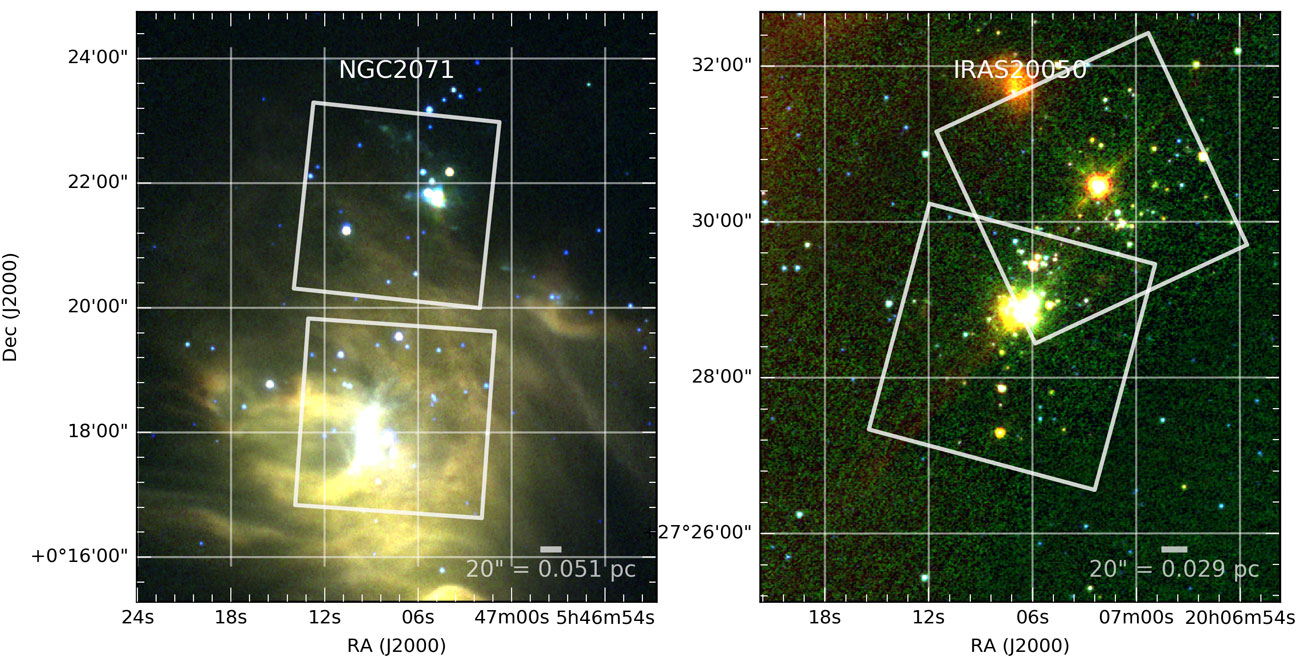
\includegraphics[width=1.5\textwidth]{Figures/NGC2071_IRAS20050_RGB.png}
\label{fig:NGC2071_IRAS20050_RGB}
\caption[NGC2071 and IRAS20050+2720]{IRAC 3-color images of NGC2071 and IRAS20050+2720. 
%\textit{Left:} The two white squares correspond to the FORCAST fields that we observed in around the core of IRAS~20050+2720. The background RGB image is a composition of \textit{Spitzer} IRAC 8~$\um$ (red), \textit{Spitzer} IRAC 5.7 $\um$ (green) , and IRAC 3.6~$\um$ (blue). The dashed red square at the center of the image correspond to the core of the cluster, displayed in greater detail in  the picture to the right. \textit{Right:} This RGB picture shows the IRAC 1, 3, and 4 bands of the core at the center of Fig.~\ref{fig:IRAS20050_RGB}. The white contours represent the contours of the FORCAST 37~$\um$ maps, and the red circles show the FORCAST-identified point sources. An infrared nebulosity can be seen to the East of the core with physical projected size of about 0.015~pc, surrounding a cavity with slightly smaller size. The nebulosity and its cavity can be seen all the way up to 37~$\um$. The far-IR emission is mapped well onto the IRAC sources, except for SOF4, for which almost no emission can be seen at shorter wavelengths. SOF4 matches the location of the bright millimeter source MMS1 \citep{Chini:2001fa}.}
}
\end{center}
\end{figure*}
\end{landscape}

\subsection{NGC 2071}
The NGC~2071 star-forming region is one of several active areas of star formation in the northern part of L1630 giant molecular cloud which is located at a distance of 390 pc \citep{A-T1982}. 
NGC~2071 itself is a reflection nebula.
The NGC~2071 infrared cluster, located about 4' north of the reflection nebula, is a region of intermediate mass star formation \citep{Strom1976, Persson1981, Butner1990}. Maps of the cloud in CO and its isotopomers \citep{Buckle2010} show a large scale clump with $\sim$1,000 M$_\odot$ associated with the cluster. Dust continuum emission at $\lambda$=0.85 and 1.3 mm peaks on center of the cluster extending ~1' in diameter containing ~30 M$_\odot$ of gas and dust \citep{Johnstone2001,Mitchell2001,Launhardt1996}. Emission from CS in the J=2-1 through J=7-6 indicate that the gas in this region is centrally condensed with a density of ~10$^6$ cm$^{-3}$ \citep{Zhou1990}. 

There are a number of near infrared surveys of the young cluster \citep[e.g.,][]{Strom1976,Lada1991,Megeath2012,Spezzi2015}. \cite{Spezzi2015} identify 52 YSOs associated with the NGC~2071 cluster, with the majority Class II sources. \cite{Flaherty2008} estimate an age of $\sim$2 Myr for the cluster, consistent with the large fraction of Class II sources (\cite{Evans2009}. The brightest far infrared emission from the cluster is associated with the IRS1 region \citep{Harvey1979,Butner1990}, which has an estimated total luminosity of 520~L$_\odot$. The immediate region of IRS 1 is, in fact, home to a number of YSOs that are infrared, X-ray, and radio sources \citep{Skinner2009,C-G2012,Kempen2012}. The radio \citep{C-G2012} and H$_2$ emission line imaging indicate that IRS~1, IRS~2, IRS~3, and, perhaps, VLA~1 are YSOs with outflows. The larger scale molecular outflow associated with this region is well studied in a number of molecules \citep{Bally1982,Chernin1993,Stoji2008}.

Figure \ref{fig:n2071overview} shows the Spitzer 3.1~$\mu$m image of the IRS~1 region on the left \citep[image from Spitzer Archive:][]{Megeath2012} and the Herschel 70~$\mu$m image on the right (image from Herschel Archive: Gould Belt Project, P.I. Andr\'e). The plus marks in both panels indicate the position of the brighter YSOs: IRS~1, IRS~2, IRS~3, IRS~4, and VLA~1. The inner red circle with a diameter of 26" indicates the extend of the saturated region in the Spitzer MIPS 24~$\mu$m image; the outer red circle, diameter 60", encompasses the region with strong imaging artifacts in the MIPS 24~$\mu$m image.
The right panel shows Herschel 70~$\mu$m image which does not resolve the emission from IRS~1, IRS~2, IRS~3, and VLA~1. The centroid of the 24~$\mu$m and 70~$\mu$m emission is between IRS~1 and VLA~1 indicating that several of the sources are contributing to the total observed emission. Interferometric observations show that the millimeter wavelength dust emission is dominated by envelopes associated with IRS~1 and IRS~3, with estimated masses of 8.2 and 12.3~M$_\odot$ material, respectively \citep{Kempen2012}. The millimeter emission also reveals the presence of disks with radii $\le$100~AU associated with IRS~1 and IRS~3 \citep{Kempen2012}.

The luminosities and masses of the individual source, IRS~1, IRS~2, IRS~3, and VLA~1, are not known. The Spectral Energy Distributions (SEDs) shortward of 10~$\mu$m support their identification as embedded YSOS \citep{Skinner2009}. \cite{Skinner2009} gives a clear discussion of the possibilities for IRS~1 and concludes that it is likely a mid-to late B~star. \cite{Kempen2012} find luminosities of 10, 3.4, and $\le$27~L$_\odot$ for IRS~1, 2, and 3, respectively, and stellar masses of $\le$1~M$_\odot$ for each, based on SED fitting. These masses and luminosities are not consistent with estimate of the total luminosity of the region of 520~L$_\odot$ \citep{Butner1990}. The far infrared images from Herschel reveal that IRS~1 alone does not totally dominate, as seen in Figure N; IRS~1, VLA~1, and IRS~3 likely make substantial contributions to the emission with lesser emission from IRS~2 and IRS~4.

\begin{landscape}
\begin{figure}
\begin{center}
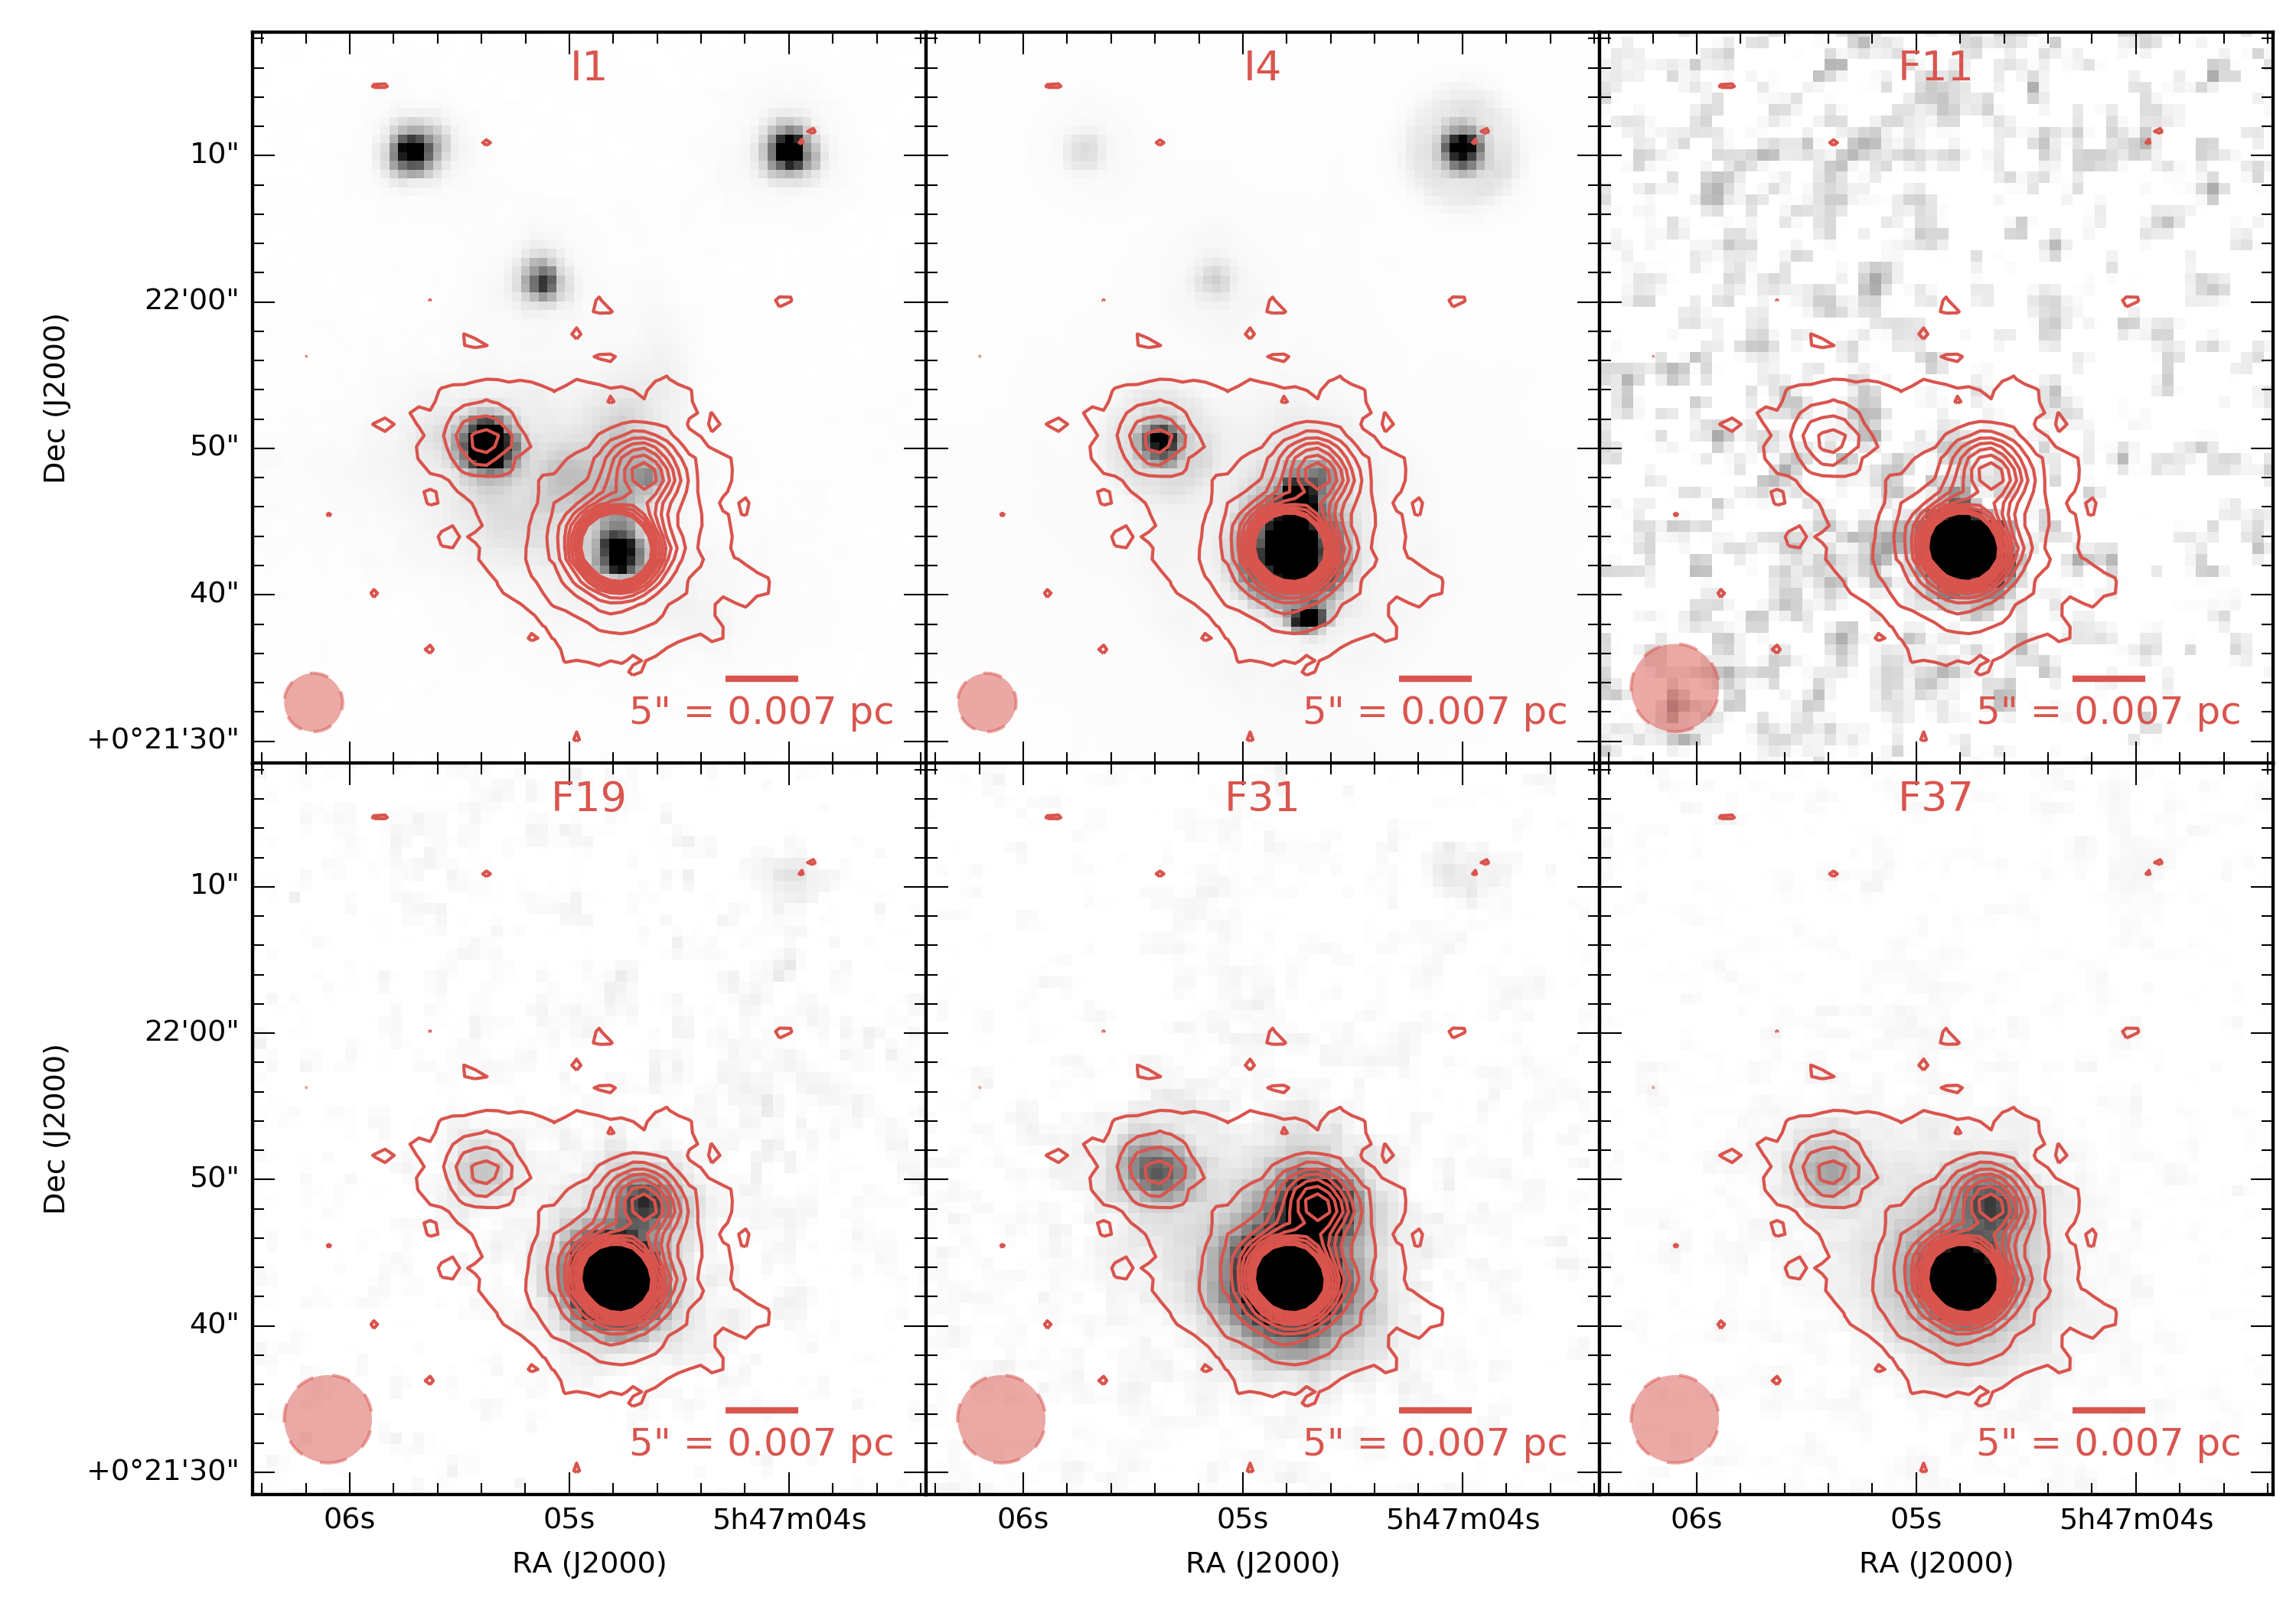
\includegraphics[width=1.5\textwidth]{Figures/NGC2071_mosaic.png}
\label{fig:NGC2071_mosaic}
\vspace{-1cm}
\caption{The core of NGC2071 is seen in two bands of the \textit{Spitzer} IRAS instrument ("I1" and "I4"), as well as with the four FORCAST bands. The increased resolution of FORCAST compared to previous instruments allows to match the long-wavelength emission with its short wavelength counterpart. The stretch in each image is adjusted for optimal readability. The white contours correspond to the FORCAST \SI{37}{\micro\meter} emission [mention the contour levels]. }
\end{center}
\end{figure}
\end{landscape}

%\section{Introduction}
%Most stars in the Galaxy form in cluster environments of sizes 2-4 pc, often containing more than 100 young stellar objects (YSOs), with typical separations of $<$0.05~pc between stars near their centers \citep{Porras:2003kxa, Allen:2007wqa, Gutermuth:2009gca}.
%Previous studies have been effective in elucidating the young stellar content and distribution in clouds on large scales (parsec down to 0.05~pc) \citep{Evans-ARAA2012}, but young cluster cores, born in dense portions of molecular clouds, are more difficult to observe. They are obscured at optical through near-IR wavelengths. At mid-IR through far-IR wavelengths, the material surrounding YSOs and involved in the stellar birth process emits due to heating by the young stars, but the resolution to date has not been sufficient to isolate individual stars in the cores of most nearby young clusters.
%
%Space telescopes such as \textit{Spitzer} and WISE have tremendous sensitivity, which made them so scientifically productive, but it limits their utility in the densest regions of star-forming clusters because of detector saturated and imaging artifacts (See \citep{2008ApJ...672.1013P} for examples). This is particularly problematic at wavelengths of \SI{24}{\micro\meter} and beyond, where a bright cluster star can dominate a region 3-5 nominal resolution elements out from the star. In fact, it is often difficult for \textit{Spitzer} and WISE to provide good flux estimates for even the brightest YSOs in the cores of clusters.
%
%The FORCAST instrument on SOFIA provides the opportunity to study cluster cores at 10 to \SI{37}{\micro\meter} with better angular resolution than \textit{Spitzer} and WISE, without saturation even on the brightest sources. Although it is less sensitive than space-based instrument at comparable wavelengths due to the large thermal background noise at 13~km altitude, FORCAST images can lift degeneracies in assigning flux by separating sources that were previously unresolved or hidden by saturation artifacts. The mid-infrared fluxes of very clustered objects are essential contraints on their YSO's spectral energy distribution (SED) which is used to determine luminosity and evolutionary state.
%
%This paper presents the results for two clusters, IRAS~200050
%and NGC~2071, which were observed as part of a FORCAST survey program to observe bright, nearby star-forming cluster cores for which the \textit{Spitzer} and WISE archival data show extensive amounts of saturation and source confusion based on near infrared images. 
%
%Section 2 provides an overview of what is know about the two clusters. In section 3, we describe our data and reduction methods in detail, and discuss systematic of the FORCAST instrument. Section 4 presents our SOFIA images and discusses them in the context of other observations. Section 5 discusses flux measurements for cluster sources at other wavelengths and outlines our procedures for deriving improved fluxes where applicable. Section 6 presents Spectral Energy Distributions and fits for the SOIFA sources, and section 7 discusses our findings.
%
%\section{Target Clusters}
%IRAS~20050+2720 and NGC~2071 are embedded young stellar clusters with total luminosities in the cores that are characteristic of intermediate mass YSOs. The following two subsections provide overviews of each cluster and its environment.
%
%\subsection{IRAS20050+2720}
%
%IRAS~20050+2720 is part of an active site of intermediate-mass star formation in the Cygnus Rift located at 700~pc \citep{Wilking:1989el}, with the particularity that it doesn't seem to contain any massive stars \citep{Gunther:2012dq}. The main cluster core is associated with water and methanol masers \citep{Palla:1991up,Fontani:2010cf} and multipolar molecular outflows observed at millimeter wavelengths \citep{Bachiller:1995cy,Anglada:1998uu,Beltran:2008gu}, suggesting that the region might have experienced a recent episode of star formation in the past 0.1 Myr which contrasts with the average age of the cluster of 1 Myr \citep{Chen:1997tb,Gutermuth:2005hx}. \cite{Gutermuth:2009gca} have identified $>170$ YSOs surrounding the core and measured their continuum fluxes up to \SI{8}{\micro\meter} with IRAC. While measurements at longer wavelengths were able to provide estimates of the total mass of the cluster \citep[e.g. using IRAS,][388~$L_\odot$]{Molinari:1996td}, the measurements are confused in the densest region and it has not been possible to properly associate the far-IR emission with its short wavelength counterpart because of the small separation between IRAC-detected protostars. The IRAS point source was classified as a luminous class 0 protostar \citep{Bachiller:1996ja}, and its emission associated with the bright millimeter source MMS1 to the northwest of the core \citep{Chini:2001fa}. \cite{Beltran:2008gu} show strong evidence that this region has multiple generations of stars, and suggest that a group of low-mass stars first completed its main accretion phase, before setting the stage for the birth of new intermediate-mass stars at the core of this cluster.
%
%We have observed two fields within the cluster (see Fig.~\ref{fig:IRAS20050_RGB}), including the brightest core at $20^h 07^m 06.70^s +\ang{27;28;54.5}$. Multiple sources in the core can be distinguished in the IRAC maps, but the core appears extended in Spitzer MIPS at \SI{24}{\micro\meter}, and is identified as a single source with WISE. No good high resolution far-infrared continuum data longward of \SI{24}{\micro\meter} was available for this source.
%
%%Cite also: \citep{Kumar:2006jo} if we want to talk about multiple generations of star formation.
%
%\begin{figure*}
%\begin{center}
%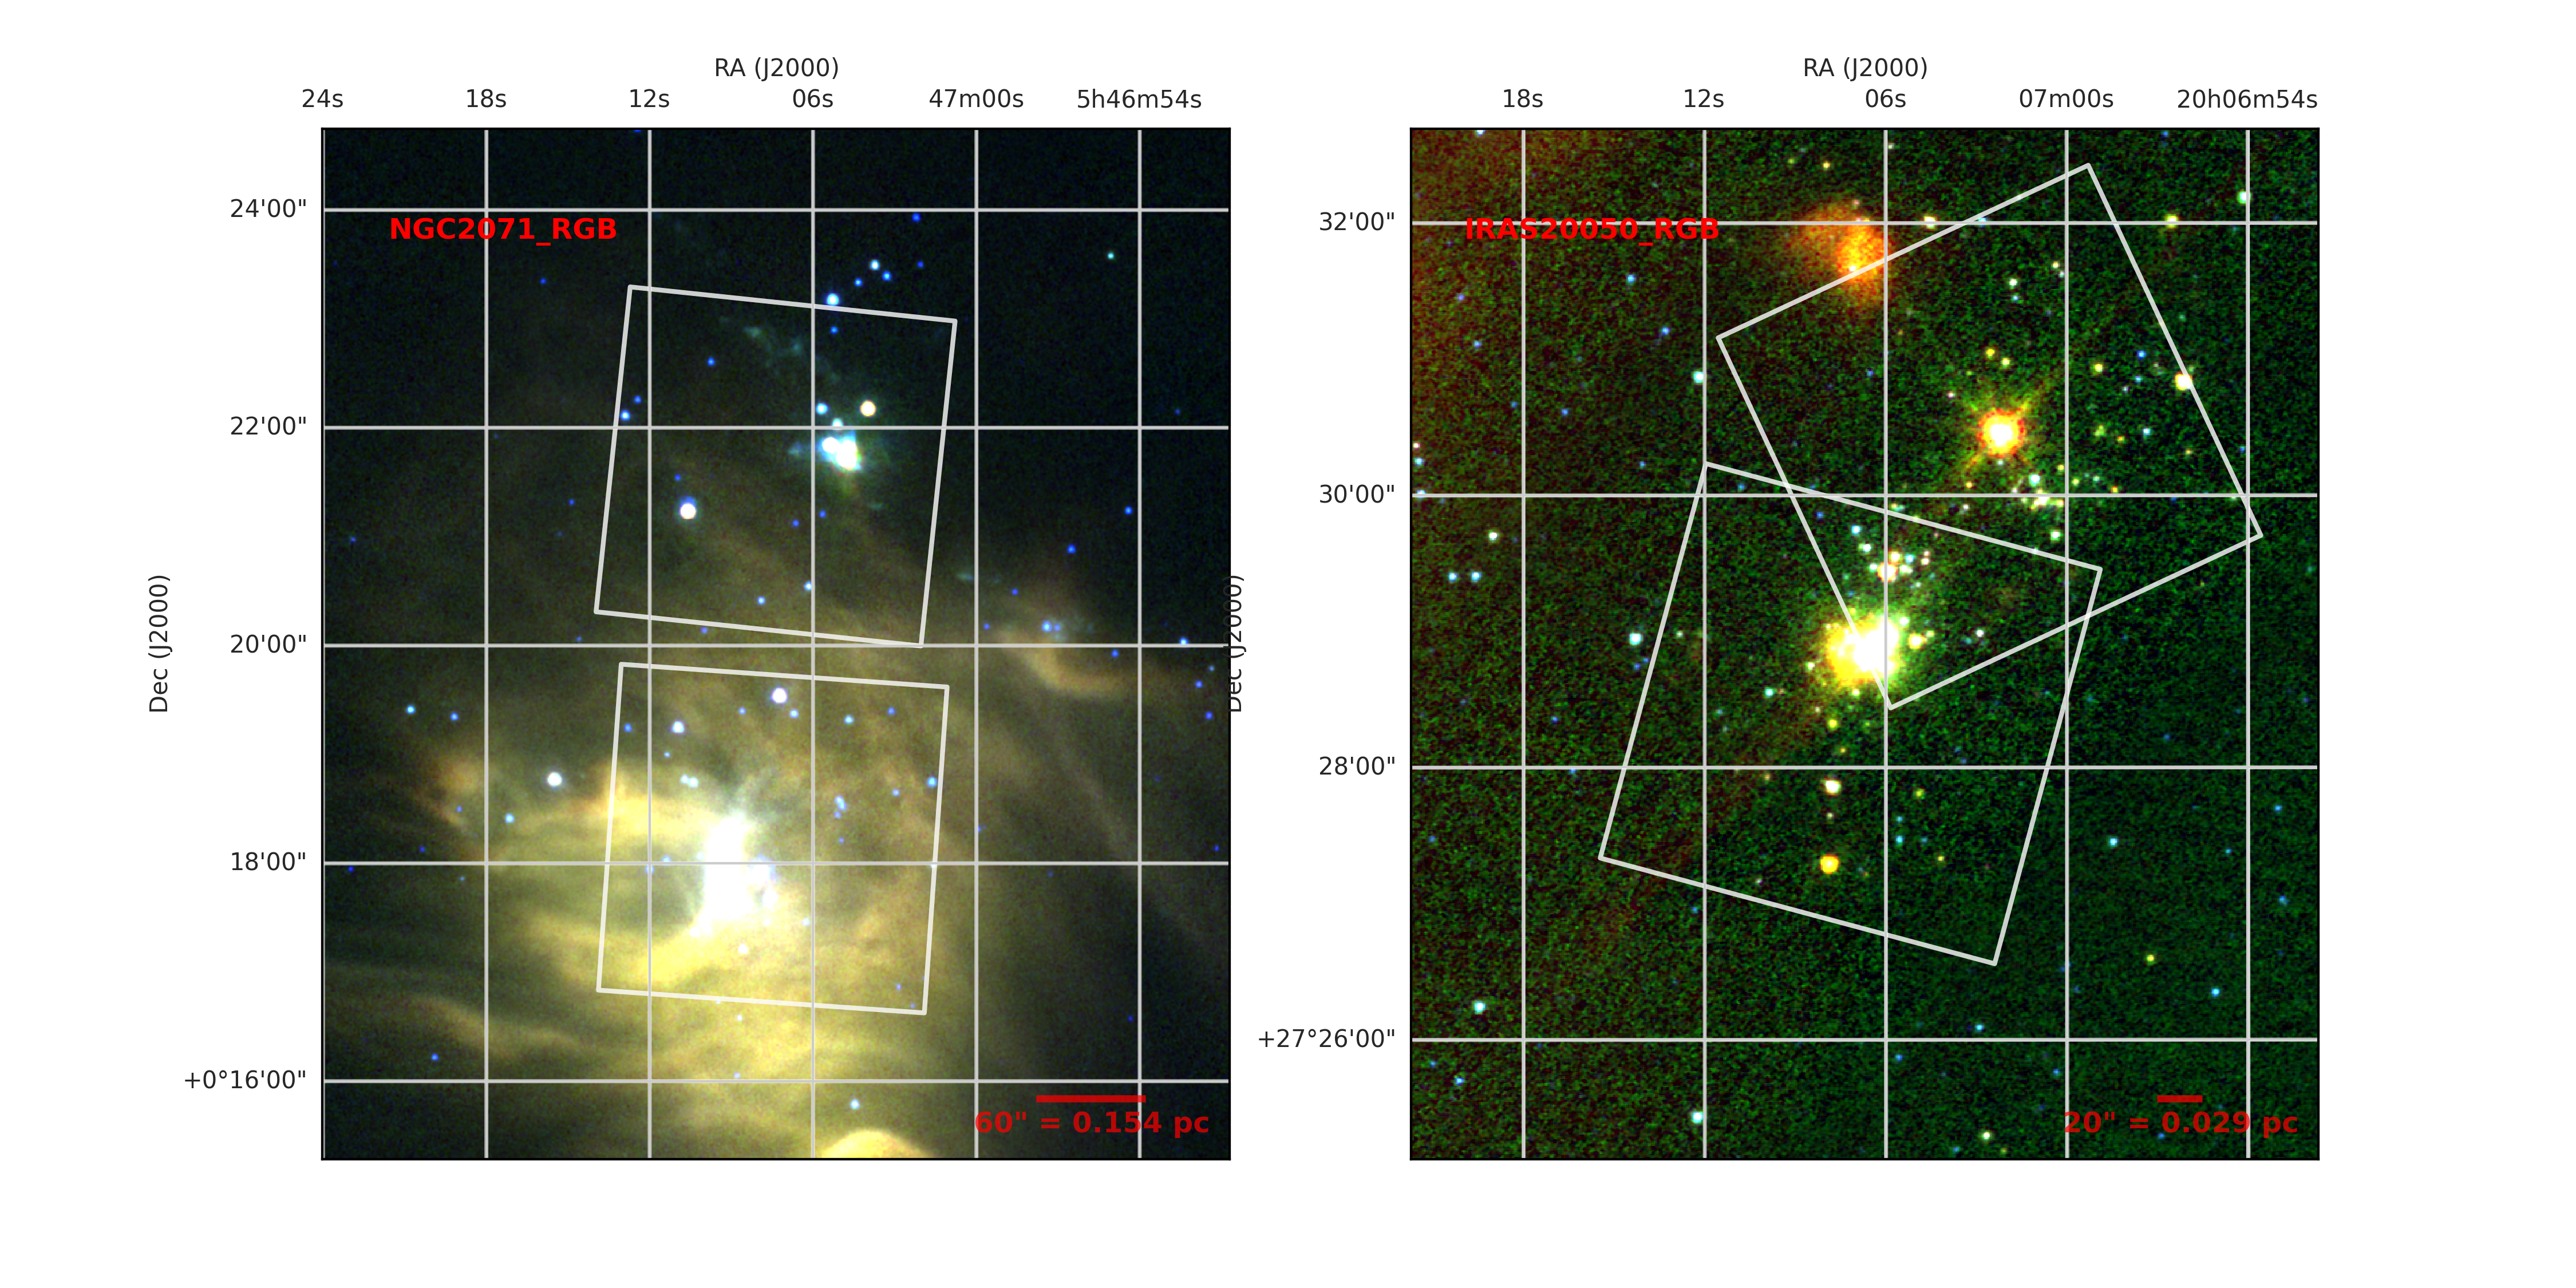
\includegraphics[width=\textwidth]{Figures/RGB.png}
%\label{fig:RGB}
%\caption{
%%\textit{Left:} The two white squares correspond to the FORCAST fields that we observed in around the core of IRAS~20050+2720. The background RGB image is a composition of \textit{Spitzer} IRAC 8~$\um$ (red), \textit{Spitzer} IRAC 5.7 $\um$ (green) , and IRAC 3.6~$\um$ (blue). The dashed red square at the center of the image correspond to the core of the cluster, displayed in greater detail in  the picture to the right. \textit{Right:} This RGB picture shows the IRAC 1, 3, and 4 bands of the core at the center of Fig.~\ref{fig:IRAS20050_RGB}. The white contours represent the contours of the FORCAST 37~$\um$ maps, and the red circles show the FORCAST-identified point sources. An infrared nebulosity can be seen to the East of the core with physical projected size of about 0.015~pc, surrounding a cavity with slightly smaller size. The nebulosity and its cavity can be seen all the way up to 37~$\um$. The far-IR emission is mapped well onto the IRAC sources, except for SOF4, for which almost no emission can be seen at shorter wavelengths. SOF4 matches the location of the bright millimeter source MMS1 \citep{Chini:2001fa}.}
%}
%\end{center}
%\end{figure*}
%
%% \begin{figure*}
%% \begin{center}
%% \includegraphics[width=5in]{}
%% \label{fig:IRAS20050_RGB_core}
%% \caption{}
%% \end{center}
%% \end{figure*}
%
%
%[Include a discussion about de-reddening towards that region?]
%
%\subsection{NGC 2071}
%The NGC~2071 star-forming region is one of several active areas of star formation in the northern part of L1630 giant molecular cloud which is located at a distance of 390 pc \citep{A-T1982}. 
%NGC~2071 itself is a reflection nebula.
%The NGC~2071 infrared cluster, located about 4' north of the reflection nebula, is a region of intermediate mass star formation \citep{Strom1976, Persson1981, Butner1990}. Maps of the cloud in CO and its isotopomers \citep{Buckle2010} show a large scale clump with $\sim$1,000 M$_\odot$ associated with the cluster. Dust continuum emission at $\lambda$=0.85 and 1.3 mm peaks on center of the cluster extending ~1' in diameter containing ~30 M$_\odot$ of gas and dust \citep{Johnstone2001,Mitchell2001,Launhardt1996}. Emission from CS in the J=2-1 through J=7-6 indicate that the gas in this region is centrally condensed with a density of ~10$^6$ cm$^{-3}$ \citep{Zhou1990}. 
%
%There are a number of near infrared surveys of the young cluster \citep[e.g.,][]{Strom1976,Lada1991,Megeath2012,Spezzi2015}. \cite{Spezzi2015} identify 52 YSOs associated with the NGC~2071 cluster, with the majority Class II sources. \cite{Flaherty2008} estimate an age of $\sim$2 Myr for the cluster, consistent with the large fraction of Class II sources (\cite{Evans2009}. The brightest far infrared emission from the cluster is associated with the IRS1 region \citep{Harvey1979,Butner1990}, which has an estimated total luminosity of 520~L$_\odot$. The immediate region of IRS 1 is, in fact, home to a number of YSOs that are infrared, X-ray, and radio sources \citep{Skinner2009,C-G2012,Kempen2012}. The radio \citep{C-G2012} and H$_2$ emission line imaging indicate that IRS~1, IRS~2, IRS~3, and, perhaps, VLA~1 are YSOs with outflows. The larger scale molecular outflow associated with this region is well studied in a number of molecules \citep{Bally1982,Chernin1993,Stoji2008}.
%\begin{figure*}
%\begin{center}
%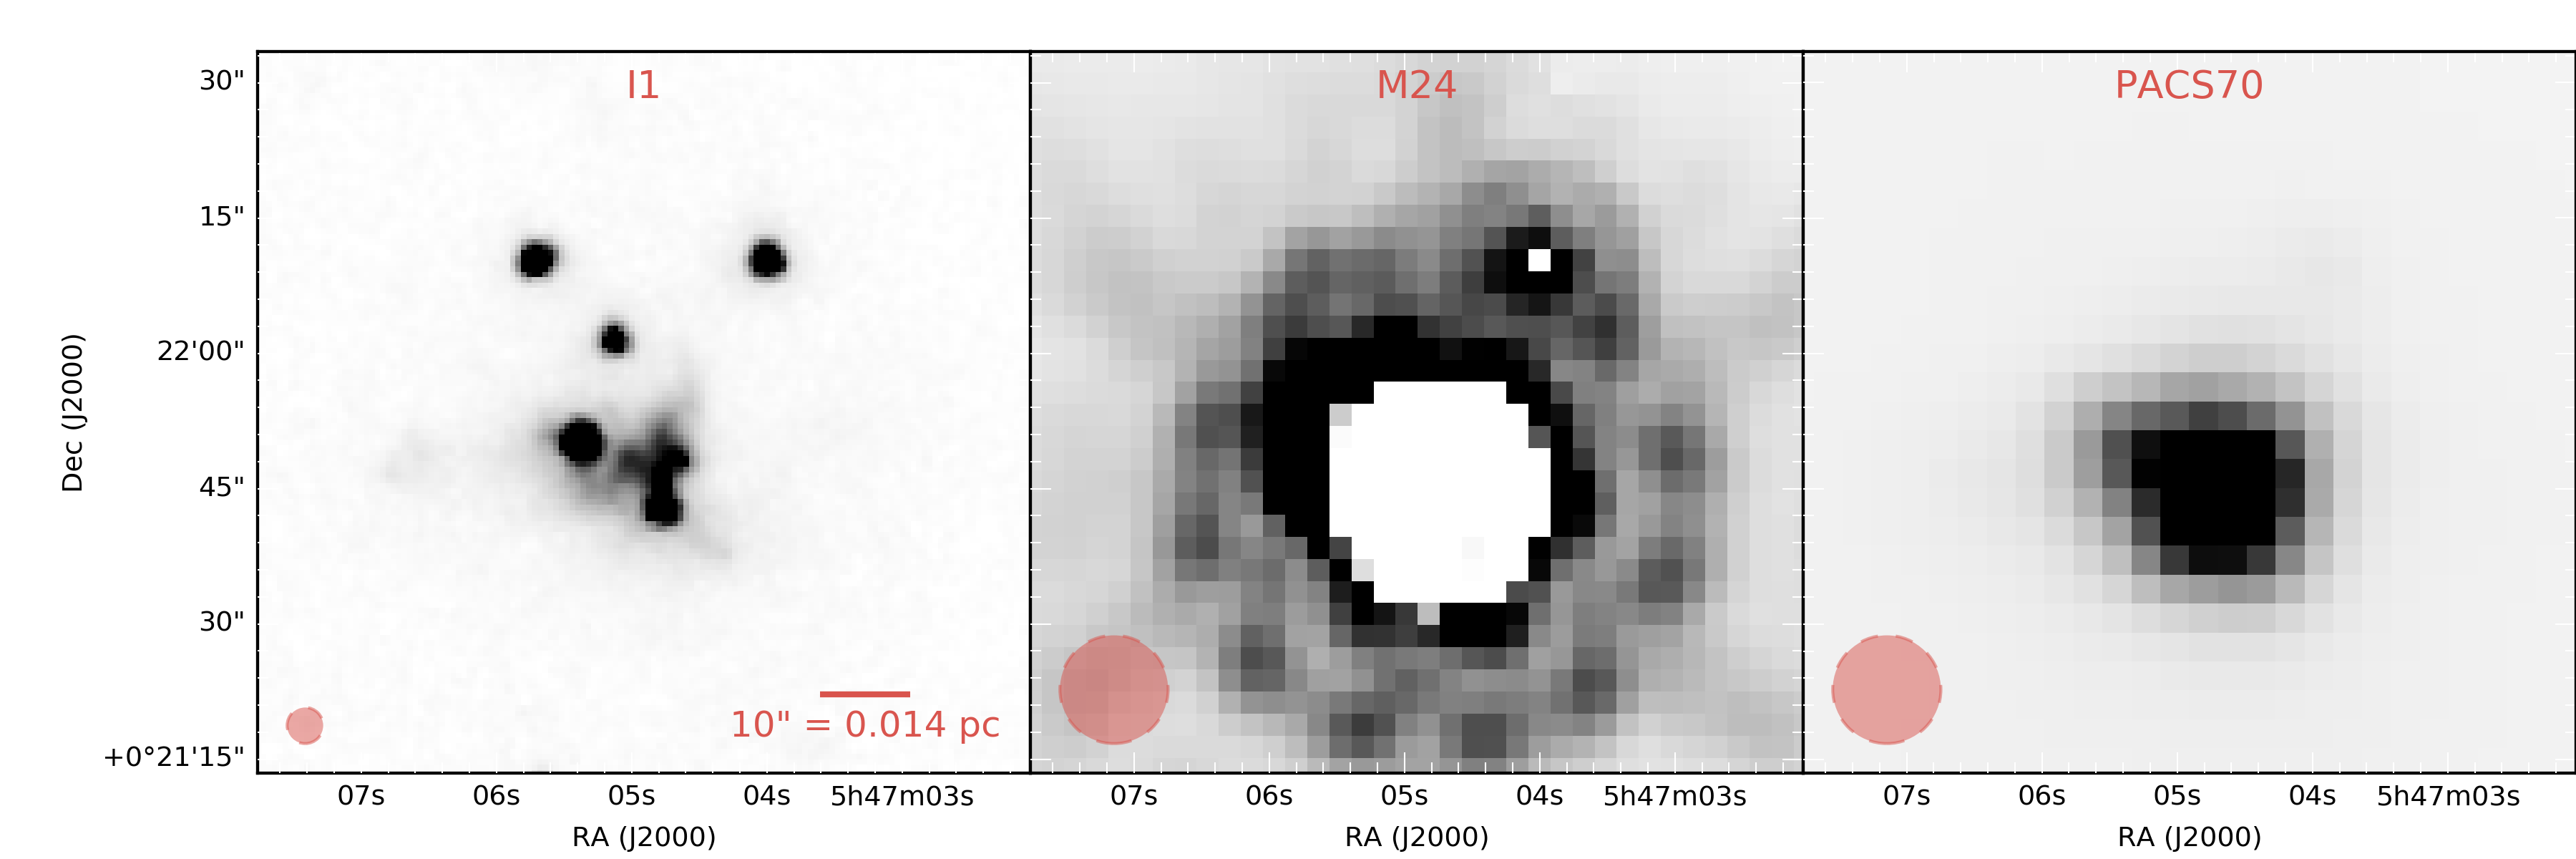
\includegraphics[width=\textwidth]{Figures/NGC2071_saturated_mosaic.png}
%\label{fig:n2071saturated}
%\caption{%NGC 2071 IRS~1 Region: The left panel show the Spitzer IRAC 3.1~$\um$ image. The right panel is the Herschel 70~$\um$ image. The green plus marks indicate the positions of IRS~1, IRS~2, IRS~3, and VLA~1. The inner red circle show the extend of the saturated region in the Spitzer MIPS 24~$\um$ image and the outer red circle encompasses the region strong affected by imaging artifacts. The gray circle on the lower right of the right panel is the resolution the 70~$\um$ image.
%NGC2071 seen with IRAC, MIPS and Herschel.}
%\end{center}
%\end{figure*}
%
%Figure \ref{fig:n2071overview} shows the Spitzer 3.1~$\mu$m image of the IRS~1 region on the left \citep[image from Spitzer Archive:][]{Megeath2012} and the Herschel 70~$\mu$m image on the right (image from Herschel Archive: Gould Belt Project, P.I. Andr\'e). The plus marks in both panels indicate the position of the brighter YSOs: IRS~1, IRS~2, IRS~3, IRS~4, and VLA~1. The inner red circle with a diameter of 26" indicates the extend of the saturated region in the Spitzer MIPS 24~$\mu$m image; the outer red circle, diameter 60", encompasses the region with strong imaging artifacts in the MIPS 24~$\mu$m image.
%The right panel shows Herschel 70~$\mu$m image which does not resolve the emission from IRS~1, IRS~2, IRS~3, and VLA~1. The centroid of the 24~$\mu$m and 70~$\mu$m emission is between IRS~1 and VLA~1 indicating that several of the sources are contributing to the total observed emission. Interferometric observations show that the millimeter wavelength dust emission is dominated by envelopes associated with IRS~1 and IRS~3, with estimated masses of 8.2 and 12.3~M$_\odot$ material, respectively \citep{Kempen2012}. The millimeter emission also reveals the presence of disks with radii $\le$100~AU associated with IRS~1 and IRS~3 \citep{Kempen2012}.
%
%The luminosities and masses of the individual source, IRS~1, IRS~2, IRS~3, and VLA~1, are not known. The Spectral Energy Distributions (SEDs) shortward of 10~$\mu$m support their identification as embedded YSOS \citep{Skinner2009}. \cite{Skinner2009} gives a clear discussion of the possibilities for IRS~1 and concludes that it is likely a mid-to late B~star. \cite{Kempen2012} find luminosities of 10, 3.4, and $\le$27~L$_\odot$ for IRS~1, 2, and 3, respectively, and stellar masses of $\le$1~M$_\odot$ for each, based on SED fitting. These masses and luminosities are not consistent with estimate of the total luminosity of the region of 520~L$_\odot$ \citep{Butner1990}. The far infrared images from Herschel reveal that IRS~1 alone does not totally dominate, as seen in Figure N; IRS~1, VLA~1, and IRS~3 likely make substantial contributions to the emission with lesser emission from IRS~2 and IRS~4.
%
%\section{SOFIA Observations}
%NGC 2071 and IRAS 200050+2720 were observed with the FORCAST instrument on SOFIA as part of a survey of selected nearby ($\le$1~kpc) bright star-forming clusters which show high protostellar density \citep{Gutermuth:2009gca} and are located in the northern hemisphere. The survey focussed on the clusters that contain one or more saturated or confused region in the archival \textit{Spitzer} and WISE data.
%
%\subsection{Data Acquisition}
%The IRAS 200050 and NGC~2071 observations were collected over three flights out of the 10-flight survey campaign. A summary is shown in Table~\ref{tab:obssummary}. Because the clusters are dominated by bright sources, the observations fit into small flight segments which filled gaps in the flight schedule. The source coordinate in Table~\ref{tab:obssummary} correspond to the centers of the green areas in Fig.~\ref{fig:IRAS20050_RGB} and Fig.~\ref{fig:n2071overview}. In each cluster, two fields separated by $\sim$ 3 arcminutes were observed to focus on two saturated regions. All fields were observed using the chop-and-node C2N mode from FORCAST, with 9-point dithering to reduce the flat field issues.
%
%%\capstartfalse
%%\begin{deluxetable*}{ccccccccccc}
%%\tablecaption{target list}
%%\tablenum{1}
%%\tablehead{\colhead{Cluster} & \colhead{RA} & \colhead{DEC} &  \colhead{Flight} & \colhead{Fields} & \colhead{Dist.} & \colhead{Time/Field} & \colhead{Sen{\_}11} & \colhead{Sen${\_}$19} & \colhead{Sen${\_}$31} & \colhead{Sen${\_}$37} \\
%%\colhead{} & \colhead{(deg)} & \colhead{(deg)} & \colhead{} & \colhead{}  & \colhead{(pc)} & \colhead{(s)} & \colhead{(Jy)} & \colhead{(Jy)} & \colhead{(Jy)} & \colhead{(Jy)}} 
%%\startdata
%%IRAS20050+2720 & 301.771 & 27.481 & F166, F131 & 2 & 700$^{1}$ & 253 & 0.026 & 0.039 & 0.068 & 0.127 \\
%%NGC2071 & 86.775 & 0.363 & F192 & 2 & 420$^{2}$ & 35 & 0.118 & 0.119 & 0.196 & 0.474
%%\enddata
%%\label{tab:obssummary}
%%\end{deluxetable*}
%%\capstarttrue 
%
%
%We observed the clusters in 4 bands: 11.1, 19.7, 31.5 and \SI{37.1}{\micro\meter}. The requested observation time in each band was calculated to detect YSOs with rising spectral energy distribution (SED) of same luminosity at the two distances of the clusters. We estimated integration time based on a rising-SED protostar model for $\sim 1.5\Lsun$. [HOW SHOULD I JUSTIFY THE FLUXES THAT WE SET AS OUR LIMITS?]
%
%Average observing time per field and average measured 1-sigma sensitivity levels are shown in Table~\ref{tab:obssummary} for the 4 bands. The measured background levels indicate the smallest detectable point source flux density at each wavelength, based on the noise measurements in the image itself. Bands 11.1 and \SI{37.1}{\micro\meter} were observed simultaneously using a dichroic filter, as were 19.7 and 31.5. However, in order to reach the required flux sensitivity for the \SI{37.1}{\micro\meter} band, we completed some of our observations with single-band observations at \SI{37.1}{\micro\meter}. 
%
%% \begin{longtable*}{ccccccc}
%% \hline
%% \hline
%% Cluster Name & Field & Field Coordinates & Band & Time (s) & Flight & Date \\
%% \hline
%
%% IRAS20050+2720 & 2 & 20h07m03s +27d30m38s & 11.1d & 135 & F131 & 2013-09-17 \\
%% IRAS20050+2720 & 2 & 20h07m03s +27d30m30s & 19.7d & 140 & F166 & 2014-05-02 \\
%% IRAS20050+2720 & 2 & 20h07m03s +27d30m47s & 31.5d & 160 & F166 & 2014-05-02 \\
%% IRAS20050+2720 & 2 & 20h07m04s +27d31m02s & 37.1d & 135 & F131 & 2013-09-17 \\
%% IRAS20050+2720 & 3 & 20h07m06s +27d28m12s & 11.1d & 135 & F166 & 2014-05-02 \\
%% IRAS20050+2720 & 3 & 20h07m06s +27d28m05s & 19.7d & 84 & F166 & 2014-05-02 \\
%% IRAS20050+2720 & 3 & 20h07m06s +27d28m13s & 31.5d & 96 & F166 & 2014-05-02 \\
%% IRAS20050+2720 & 3 & 20h07m06s +27d28m06s & 37.1d & 126 & F166 & 2014-05-02 \\
%% \hline
%
%% NGC2071 & 1 & 05h47m07s +00d17m49s & 11.1d & 18 & F192 & 2015-02-05 \\
%% NGC2071 & 1 & 05h47m07s +00d18m02s & 19.7d & 11 & F192 & 2015-02-05 \\
%% NGC2071 & 1 & 05h47m06s +00d17m55s & 31.5d & 11 & F192 & 2015-02-05 \\
%% NGC2071 & 1 & 05h47m07s +00d18m03s & 37.1d & 21 & F192 & 2015-02-05 \\
%% NGC2071 & 2 & 05h47m07s +00d21m30s & 11.1d & 18 & F192 & 2015-02-05 \\
%% NGC2071 & 2 & 05h47m07s +00d21m31s & 19.7d & 18 & F192 & 2015-02-05 \\
%% NGC2071 & 2 & 05h47m07s +00d21m34s & 31.5d & 24 & F192 & 2015-02-05 \\
%% NGC2071 & 2 & 05h47m07s +00d21m34s & 37.1d & 21 & F192 & 2015-02-05 \\
%
%% \caption{List of observations}
%% \end{longtable*}
%
%%Make sure to mention the distances picked and the references for it, as well as the cluster's age estimate
%%Need to find references to cite for details about each region
%\subsection{Data reduction}
%The data are processed through various versions of the online pipeline to yield Level 2 data products available on the archive \citep{Herter:2013by}. We apply our own reduction procedure and photometry pipeline on those products to derive final images, source positions, fluxes and sensitivities. The software utilizes the Python \textit{astropy} package \citep{2013A&A...558A..33A} and its associated modules \textit{photutils} and \textit{APLpy}. 
%
%\subsubsection{Pre-treatment}
%Some manual treatment of each image is necessary before it can be analyzed by our software, which follows this procedure: a) visually aligning the WCS coordinate system, often 10-20" off, using point sources and archival data from other wavelengths and facilities such as IRAC \SI{8}{\micro\meter}; b) cropping the images to clean off the nodded fields, and c) identify the coordinates of each source, both point-like and extended.
%
%After these manual steps, the Level 2 images are multiplied by the calibration factor provided by the online pipeline, which converts them to Jy/pixel. We do not proceed to any systematic color correction, but the effects on the fluxes are very small \citep{Herter:2013by}.
%\begin{comment}
%\begin{enumerate}
%\item Adjust WCS coordinates: use images at other wavelengths (2MASS, IRAC, MIPS, WISE) to re-align the (RA, DEC) position of the field. We estimate that this process is good to within one SOFIA pixel (0.768") for the fields where one or more point sources can be identified. Extended fields are less trustworthy, since matching the extended emission to other wavelengths is harder. The rotation of the field produced by the SOFIA pipeline is correct for all of our data. 
%\item Crop each image, remove chopped fields, remove artifacts.
%\item Identify and categorize sources: isolated point sources, clustered point sources, and extended sources. For extended sources, a circular or elliptical aperture is used to try to encompass the entirety of the emission.
%\item Manually identify a location in the field that corresponds to a representative background.
%\end{enumerate}
%\end{comment}
%\subsubsection{Source flux extraction and calibration}
%\begin{comment}
%We feed the adjusted FITS and associated metadata files to a photometry pipeline. The pipeline first processes all the calibrator stars that are observed during each flight, with each filter setting, and derives a new aperture correction factor for each image, based on an aperture of 4 pixels radius (3.072") and an aperture of 12 pixels radius. We consider that the latter aperture contains all the flux from a given point source.
%
%We distinguish between 3 types of sources after manual identification: \textit{isolated}, which are point sources with no nearby objects; \textit{clustered}, which are point sources with nearby objects; and \textit{extended}, which are not consistent with being point sources. [THIS PARAGRAPH MAY GO AWAY IF WE DON'T WANT TO TALK ABOUT GENERALITIES ABOUT THE PIPELINE]
%
%
%For point sources, we use our standard aperture of 4 pixels at all wavelengths. We consider an annulus surrounding the source extending from 12 to 20 pixels radius (24 to 40 for clustered sources): the local background is determined from the mode of the pixels in the annulus, while the sensitivity is calculated by measuring the standard deviation of 4-pixel apertures within that annulus [Cite Taro's paper and the Herschel photometry paper that Tracy gave us]. We apply the aperture correction derived from the calibrator observations taking during that flight.
%
%For extended sources, an elliptical aperture is determined manually from the \SI{37}{\micro\meter} images. The local background is determined from the mode of an elliptical annulus, with an inner boundary at the elliptical aperture and an outer boundary corresponding to an ellipse 20\% larger. The sensitivity quoted is the point source sensitivity, and is determined following the same method as for point sources, using the standard deviation of apertures spread across the elliptical annulus. [NO NEED TO MENTION THIS SINCE WE MIGHT NOT TREAT EXTENDED SOURCES]
%
%The photometry from sources that were observed in different flights is then combined to increase the signal-to-noise ratio. This combination takes into account the sensitivity of each source by appropriately weighing each image.
%
%Although we can compute source sensitivities based on the local noise, and we use the calibrators each flight to determine the aperture correction, observations with SOFIA have additional noise from the water vapor overburden and air mass, as well as from the flat field variations. These noise contributions usually amount to much higher than the sensitivities estimated from the local background, and we follow the recommendation from \citep{Herter:2012hv} to adopt a 20\% uncertainty for our flux estimates. 
%
%\end{comment}
%
%\subsection{Photometry at other wavelengths}
%
%\subsection{Instrumental Characterization}
%[THIS WHOLE DISCUSSION MIGHT FIT BETTER IN THE PAPER ABOUT THE WHOLE SURVEY, RATHER THAN THIS PAPER WHICH IS JUST ABOUT TWO CLUSTERS...]
%The three flights discussed here were part of the total of 10 data flights for the entire survey. The larger context of the entire survey allowed us to follow the evolution of the instrument properties throughout the two years of science observations. We discuss three metrics: the evolution of the aperture correction factor, the evolution of the instrument's residuals, and the evolution of the PSF size, through half width at half max of the encircled energy distribution, that we call $\Rfifty$. This is done in an attempt to assess the uncertainties in our flux determination, and our confidence in determining that sources are point-like or extended. %This study is based  on the large number of calibrator observations during our 10 science flights.
%
%\subsubsection{PSF size}
%
%Fig~\ref{fig:average_EE} shows the average of the normalized encircled energy distribution of the PSF, measured on all the calibrators of our sample. Each curve represents one of the five different combinations of bandpass filter and dichroic setting that we use for our observations: \SI{11.1}{\micro\meter}, \SI{19.7}{\micro\meter}, \SI{31.5}{\micro\meter}, \SI{37.1}{\micro\meter} with dichroic and \SI{37.1}{\micro\meter} without a dichroic (open). 
%
%As expected, the PSF at \SI{37.1}{\micro\meter} is larger than the PSFs at shorter wavelengths, but less that the traditional diffraction limit rule. This indicates that additional PSF smearing is occurring at short wavelengths, likely due to plane jitter and pointing errors. This was predicted and mentioned in the SOFIA Observer's Handbook. Throughout all the flights, the largest 1-sigma error occurs for the \SI{37}{\micro\meter} observations at about XX\%. CONCLUDE ON OUR ABILITY TO DETERMINE WHETHER A SOURCE IS EXTENDED OR NOT.
%
%To look at the behavior of the PSF in more detail, we can use the half width at half maximum of the encircled energy distribution, $\Rfifty$ as a proxy for PSF size. The variation of this quantity for the various flights, bandpass/dichroic setting, and calibrators used is showed in Fig~\ref{fig:Rfifty_dist}. This shows the flight-to-flight differences and, for some calibrators, the in-flight variability. We find that the latter is usually NN\% or less, except for the SOFIA flight on 05-02-2014, for which the spread is quite considerable. The variation from flight to flight is larger than the variation within a given flight, which indicates variability in the observing conditions, systematics, or thermal radiation environment of the observatory between different flights. Hence, we conclude that the extension of a source can be best determined by comparing $\Rfifty$ for that source with $\Rfifty$ for the corresponding calibrator measurement for that flight and dichroic setting, to within NN\%, 1-sigma confidence.
%\begin{figure}
%\begin{center}
%
%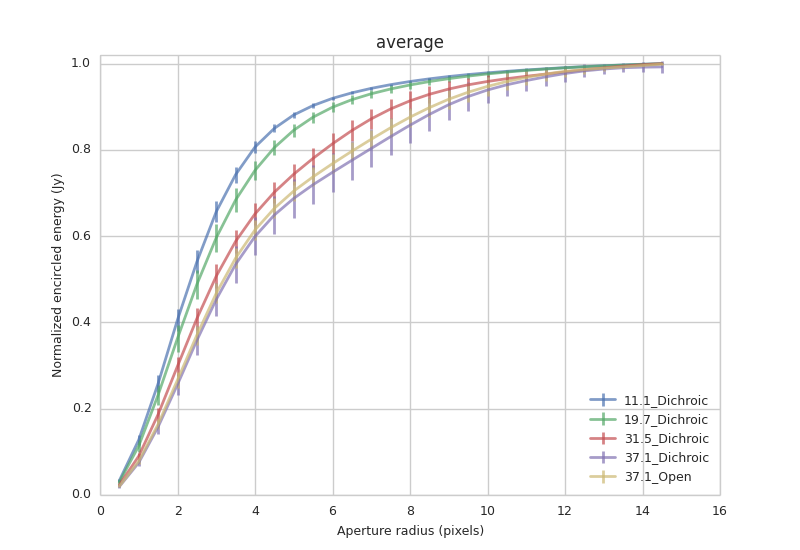
\includegraphics[width=0.45\textwidth]{Figures/average.png}
%\label{fig:average_EE}
%\caption{PSF size distribution}
%\end{center}
%\end{figure}
%
%\begin{figure}
%\begin{center}
%
%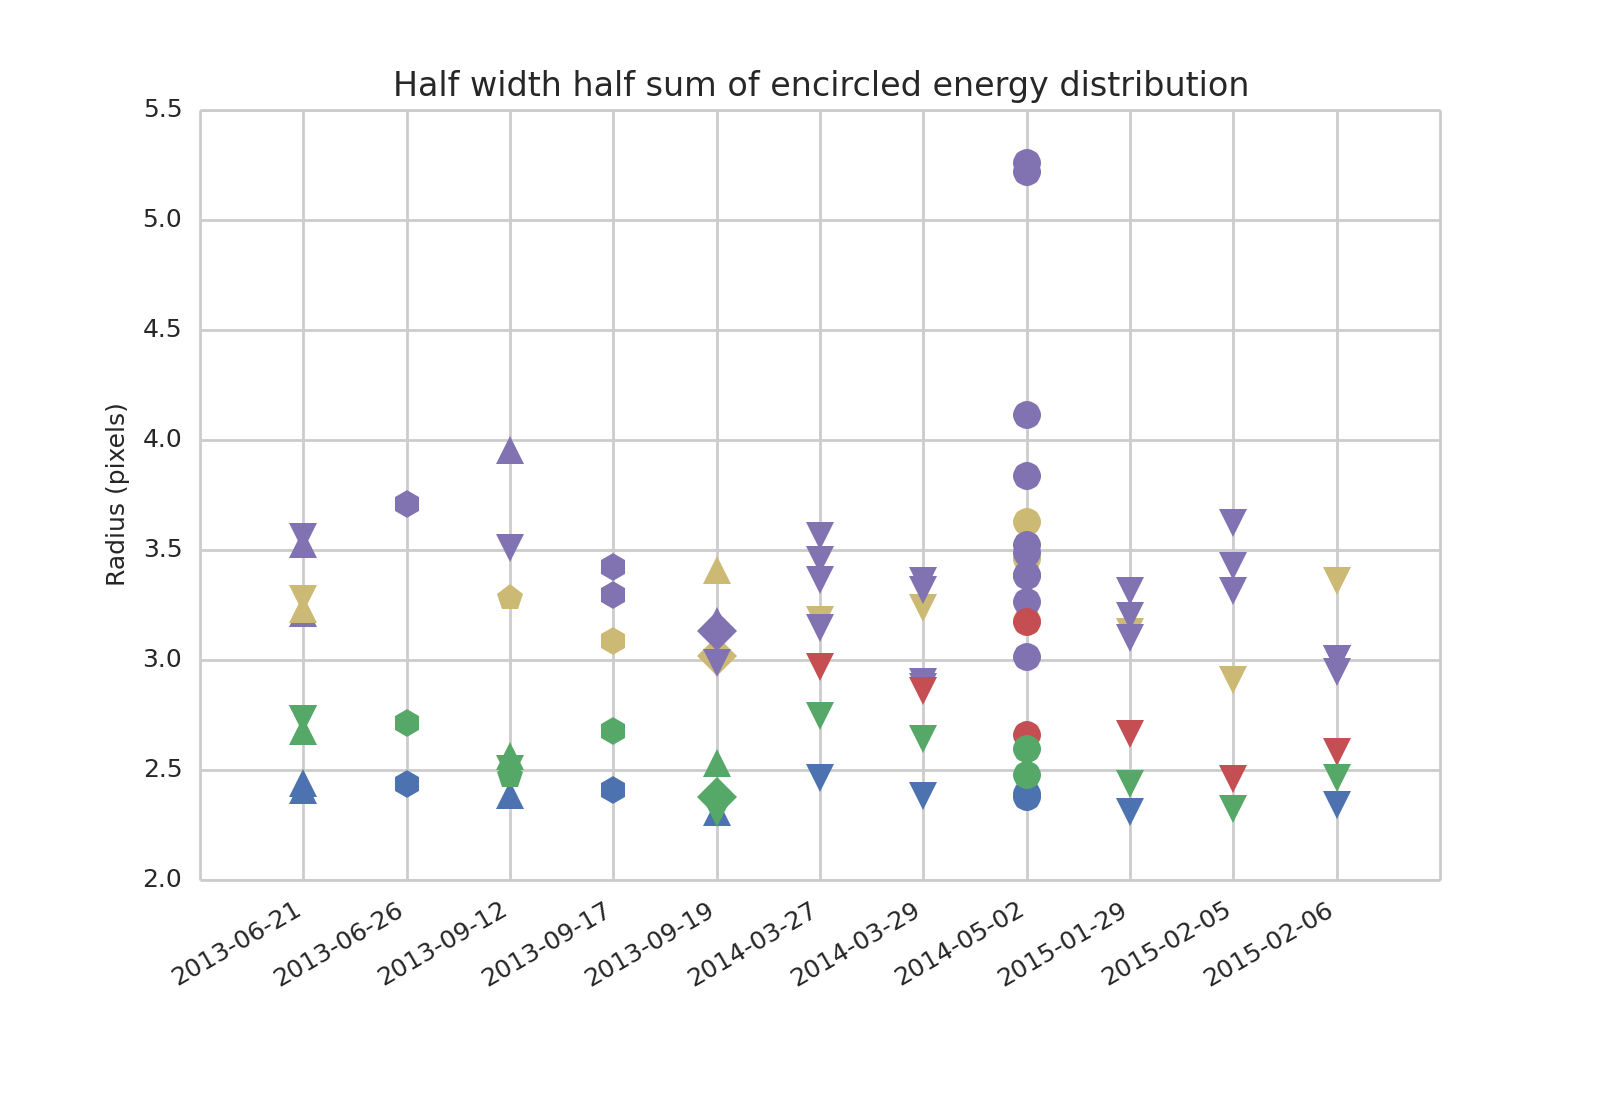
\includegraphics[width=0.45\textwidth]{Figures/fwhs.png}
%\label{fig:Rfifty_dist}
%
%\caption{PSF size distribution}
%\end{center}
%\end{figure}
%
%\subsubsection{Aperture correction}
%In Fig~\ref{fig:response}, we plot the aperture correction factor that we compute from the ratio of the flux measured within an aperture of 4 pixels, divided by the flux measured in an aperture of 12 pixel radius, which we consider to be encompassing the total flux in the source. Not surprisingly, this graph follows very closely the plot of $\Rfifty$ shown in Fig~\ref{fig:Rfifty_dist}, showing the close link between the aperture correction factor and the shape of the calibrator's PSF. For the aperture correction variability, we adopt a XX, 1-sigma uncertainty value on the flux estimate.
%
%
%
%\subsubsection{Instrument response}
%To further study the variability of the observing, we can look at the detector response and the aperture correction evolution after applying the calibration factor. In the ideal conditions, the calibration factor always leads to the same flux measurement of the calibrator source, within the pipeline's systematic errors and residual noise. The detector response is measured here by simply applying aperture photometry on the calibrators to measure their fluxes, using the same local background subtraction as the one described in the previous sections. Calibrator stars are good ways to correct for telescope and atmospheric variability, as their far-infrared fluxes are not expected to vary significantly over any relevant timescale. %We adopt a value of XX, 1-sigma value for the response variability, effectively representing the uncertainties in the observatory and the atmosphere.
%In Fig~\ref{fig:response}, we plot all the measured fluxes of the calibrators. The flux variability from flight to flight for a given calibrator is small (typically [CALCULATE THIS]), and the variability within the same flight is even smaller [QUANTIFY]. We adopt a XX, 1-sigma uncertainty value for the absolute flux measurement. This is the residual uncertainty after applying the systematic correction produced by the SOFIA FORCAST online pipeline.
%
%
%
%\begin{figure}
%\begin{center}
%
%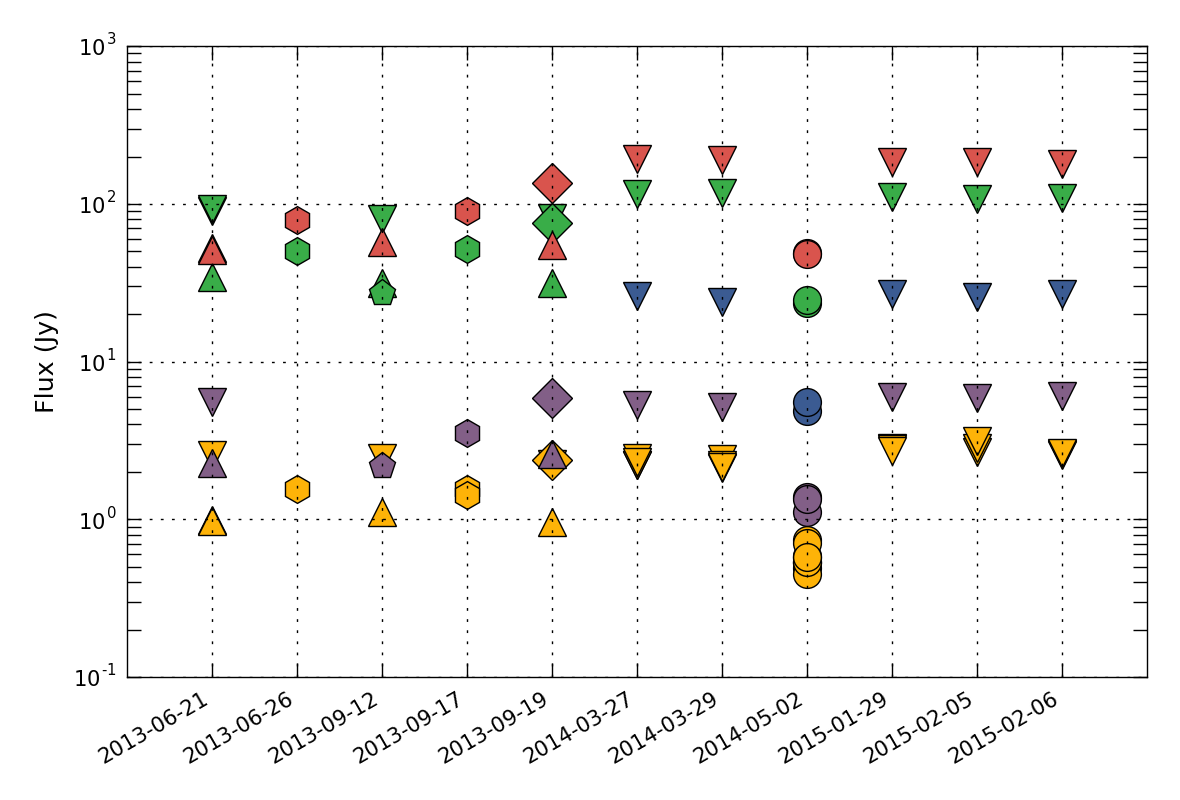
\includegraphics[width=0.45\textwidth]{Figures/Phot_val.png}
%\label{fig:response}
%\caption{Instrumental response and aperture correction}
%
%\end{center}
%\end{figure}
%
%\begin{figure}
%\begin{center}
%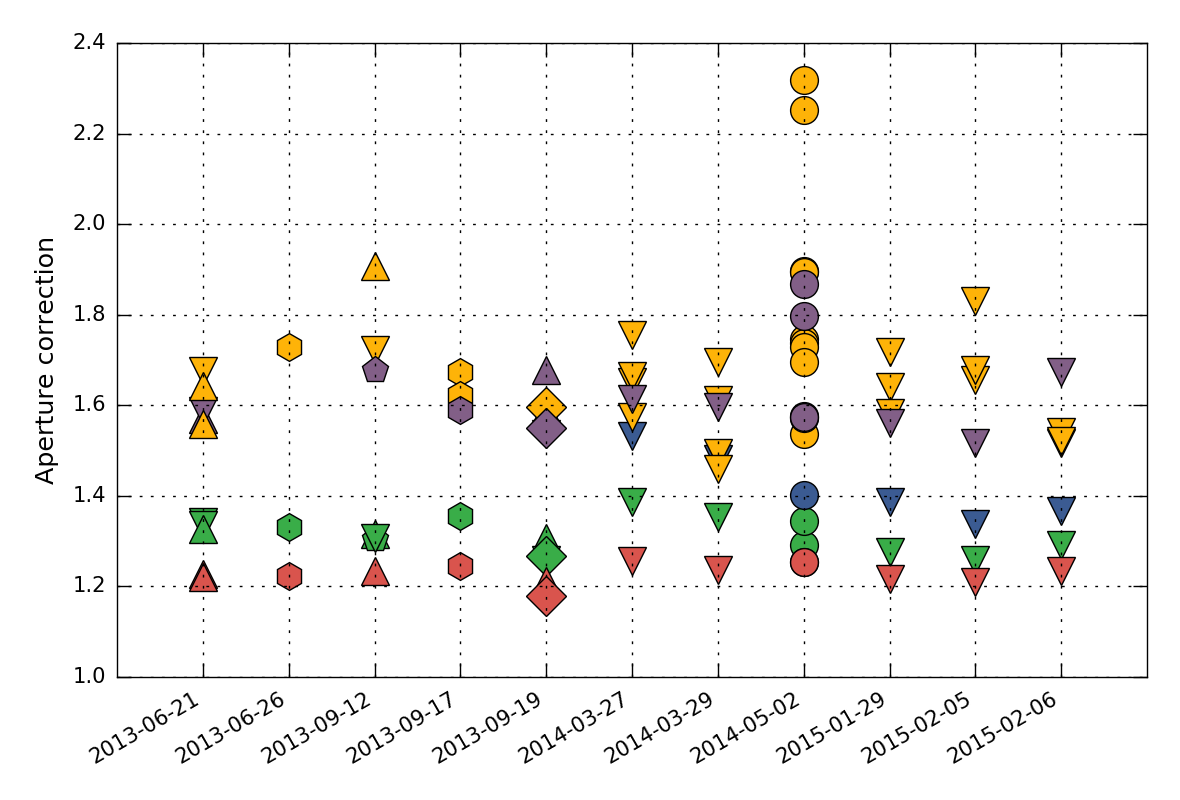
\includegraphics[width=0.45\textwidth]{Figures/Aper_corr.png}
%\label{fig:aper_corr}
%
%\caption{Instrumental response and aperture correction}
%\end{center}
%\end{figure}
%
%%WHAT IS THE BOTTOM LINE FROM THIS DISCUSSION? IS A FLUX MEASUUREMENT LIMITED BY VARIATIONS IN THE PSF IF IT IS BRIGHT? SOMETHING ELSE? IT SEEMS LIKE THE CONCLUSION FROM THIS SECTION SHOULD BE A STATEMENT ABOUT THE SYSTEMATIC ERRORS ON ANY QUOTED FLUX MEASUREMENT AND A STATEMENT ABOUT LIMITATIONS ON KNOWING WHETHER A SOURCE IS EXTENDED RELATIVE TO A POINT SOURCE.
%\section{Observational results}
%\subsection{IRAS 200050}
%
%SOFIA photometry results, IRAC photometry issues and results; looking at the sources that are fit by guthermuth, we find a 10\% agreement between our photometry results and theirs.
%
%\subsubsection{Photometry results and maps}
%
%\subsubsection{SEDs}
%
%
%\subsubsection{Upper limits on other sources in the field}
%
%
%\begin{figure}
%\begin{center}
%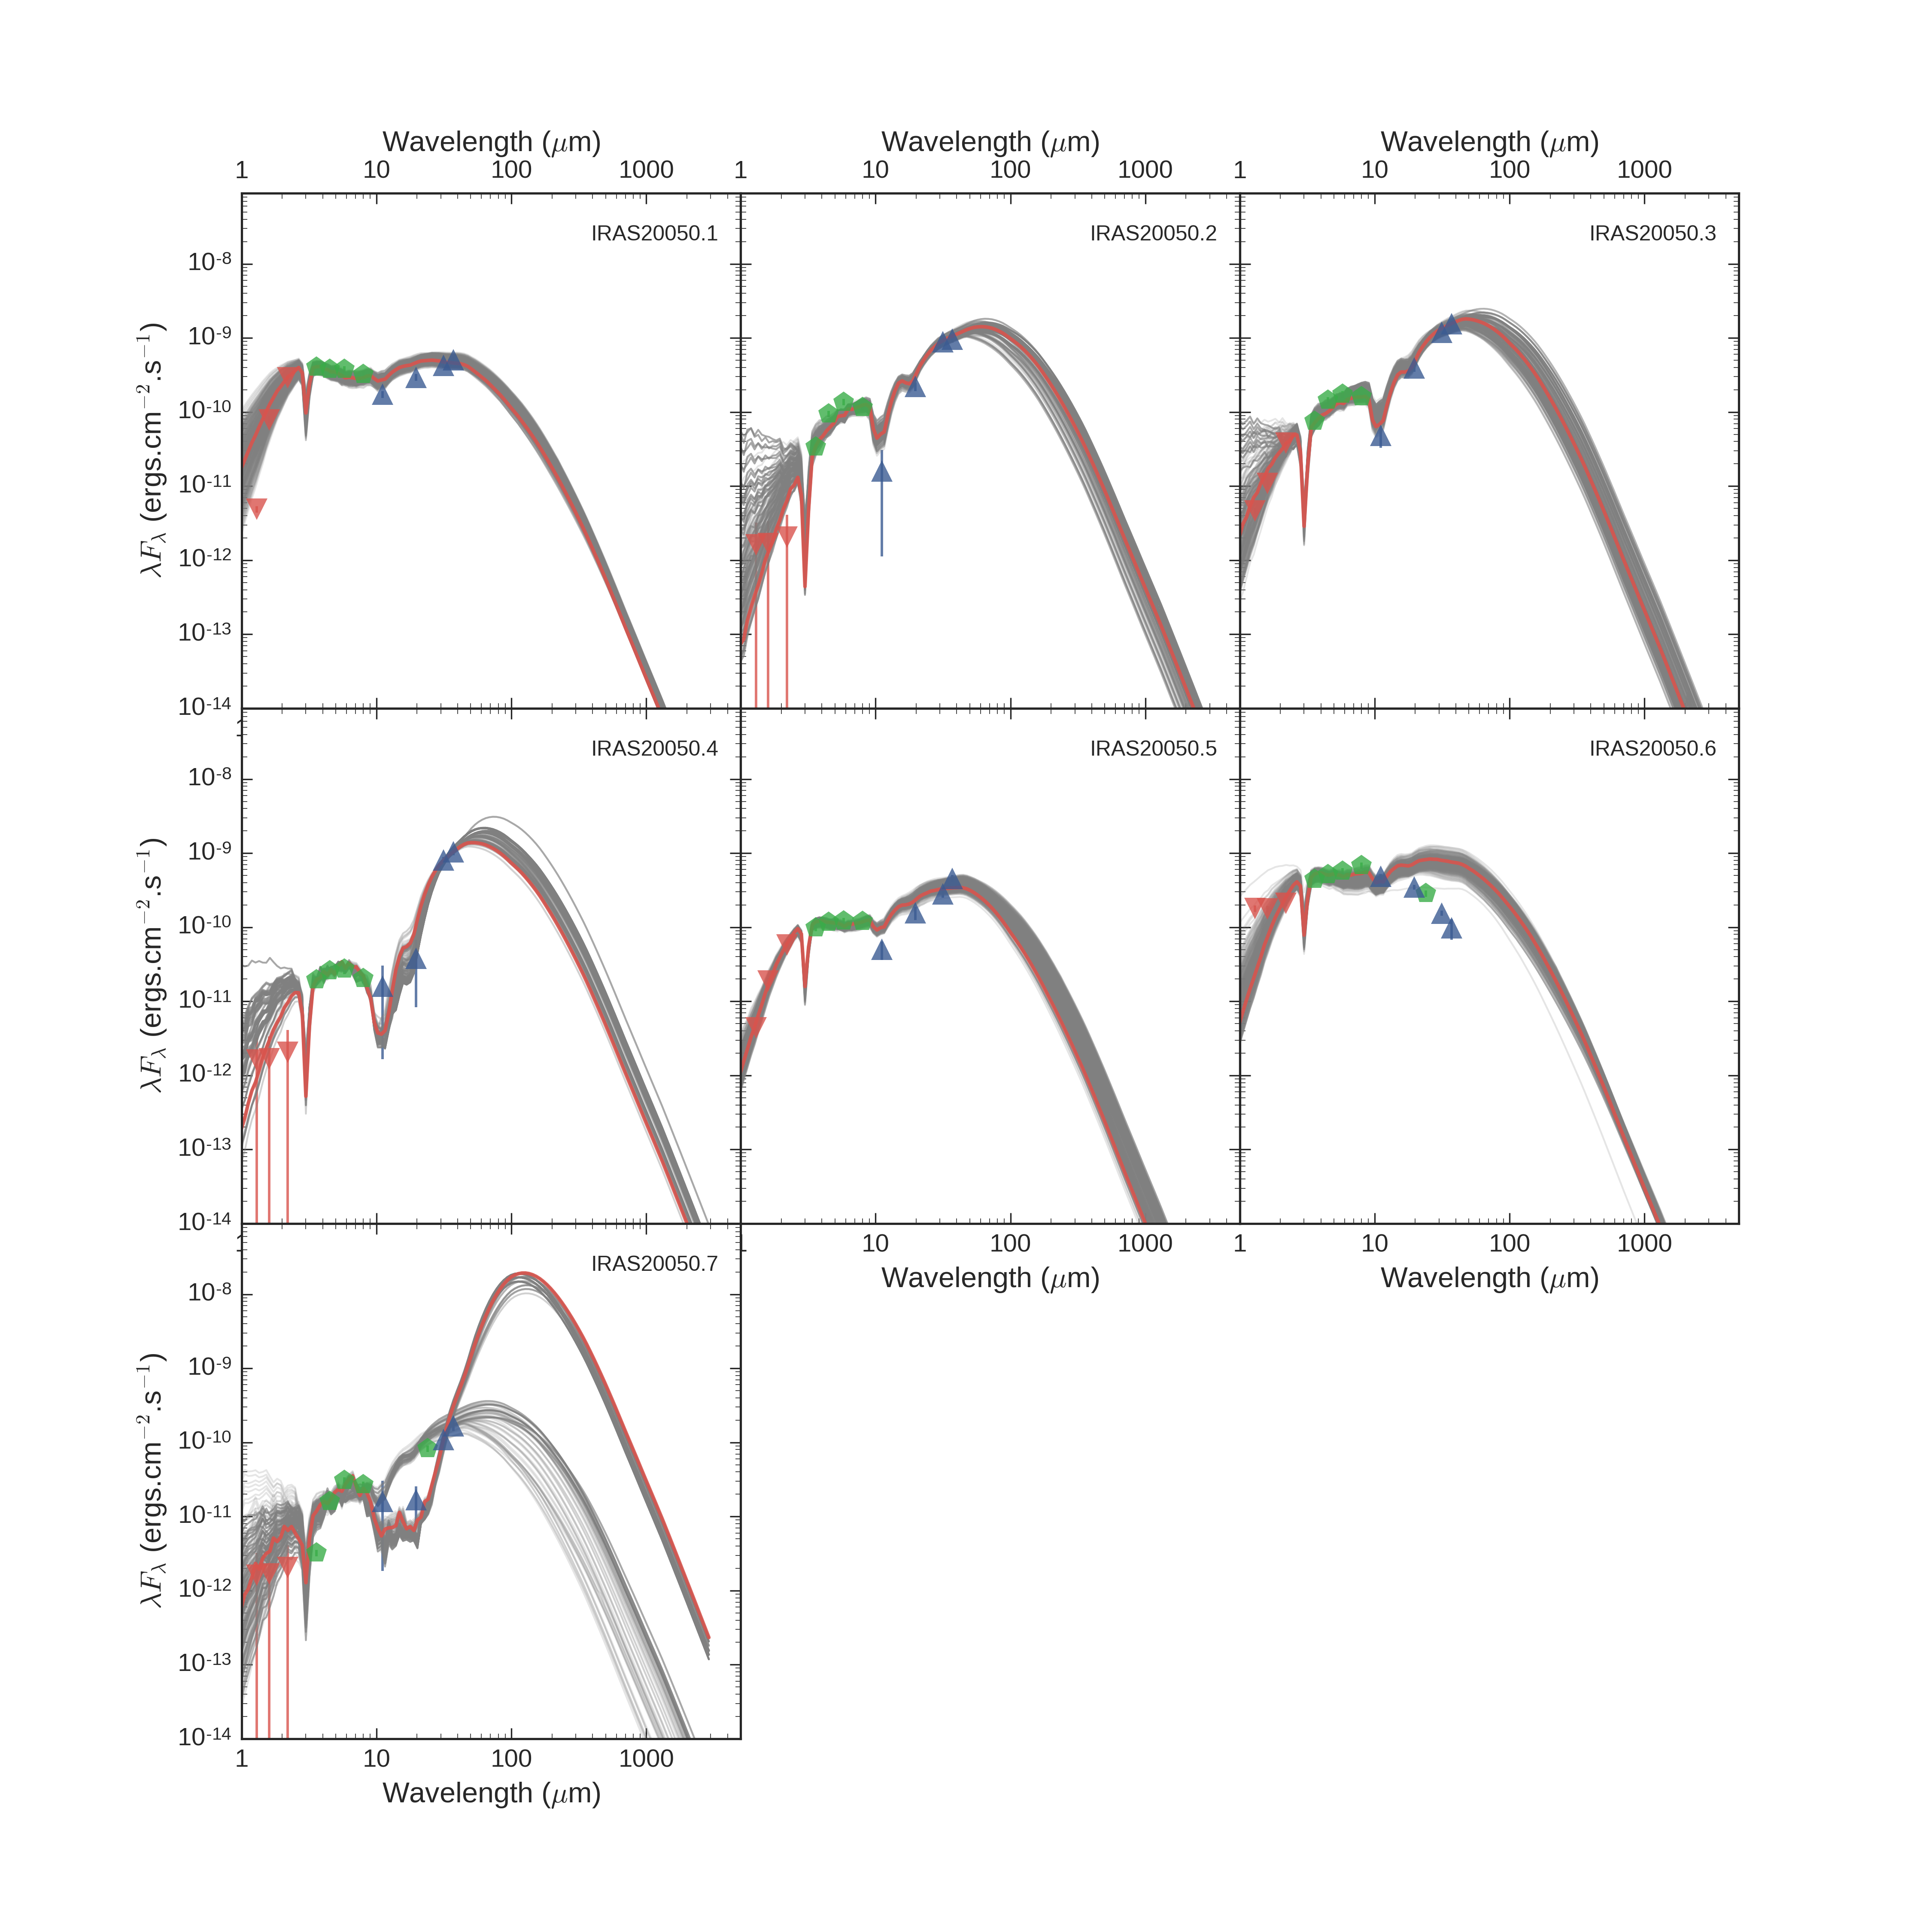
\includegraphics[width=1\textwidth]{Figures/IRAS20050_SEDs.png}
%\label{fig:IRAS20050_SEDs}
%\caption{}
%\end{center}
%\end{figure}
%
%
%
%
%\subsection{NGC2071}
%
%
%\subsubsection{Photometry results and maps}
%
%\begin{figure}
%\begin{center}
%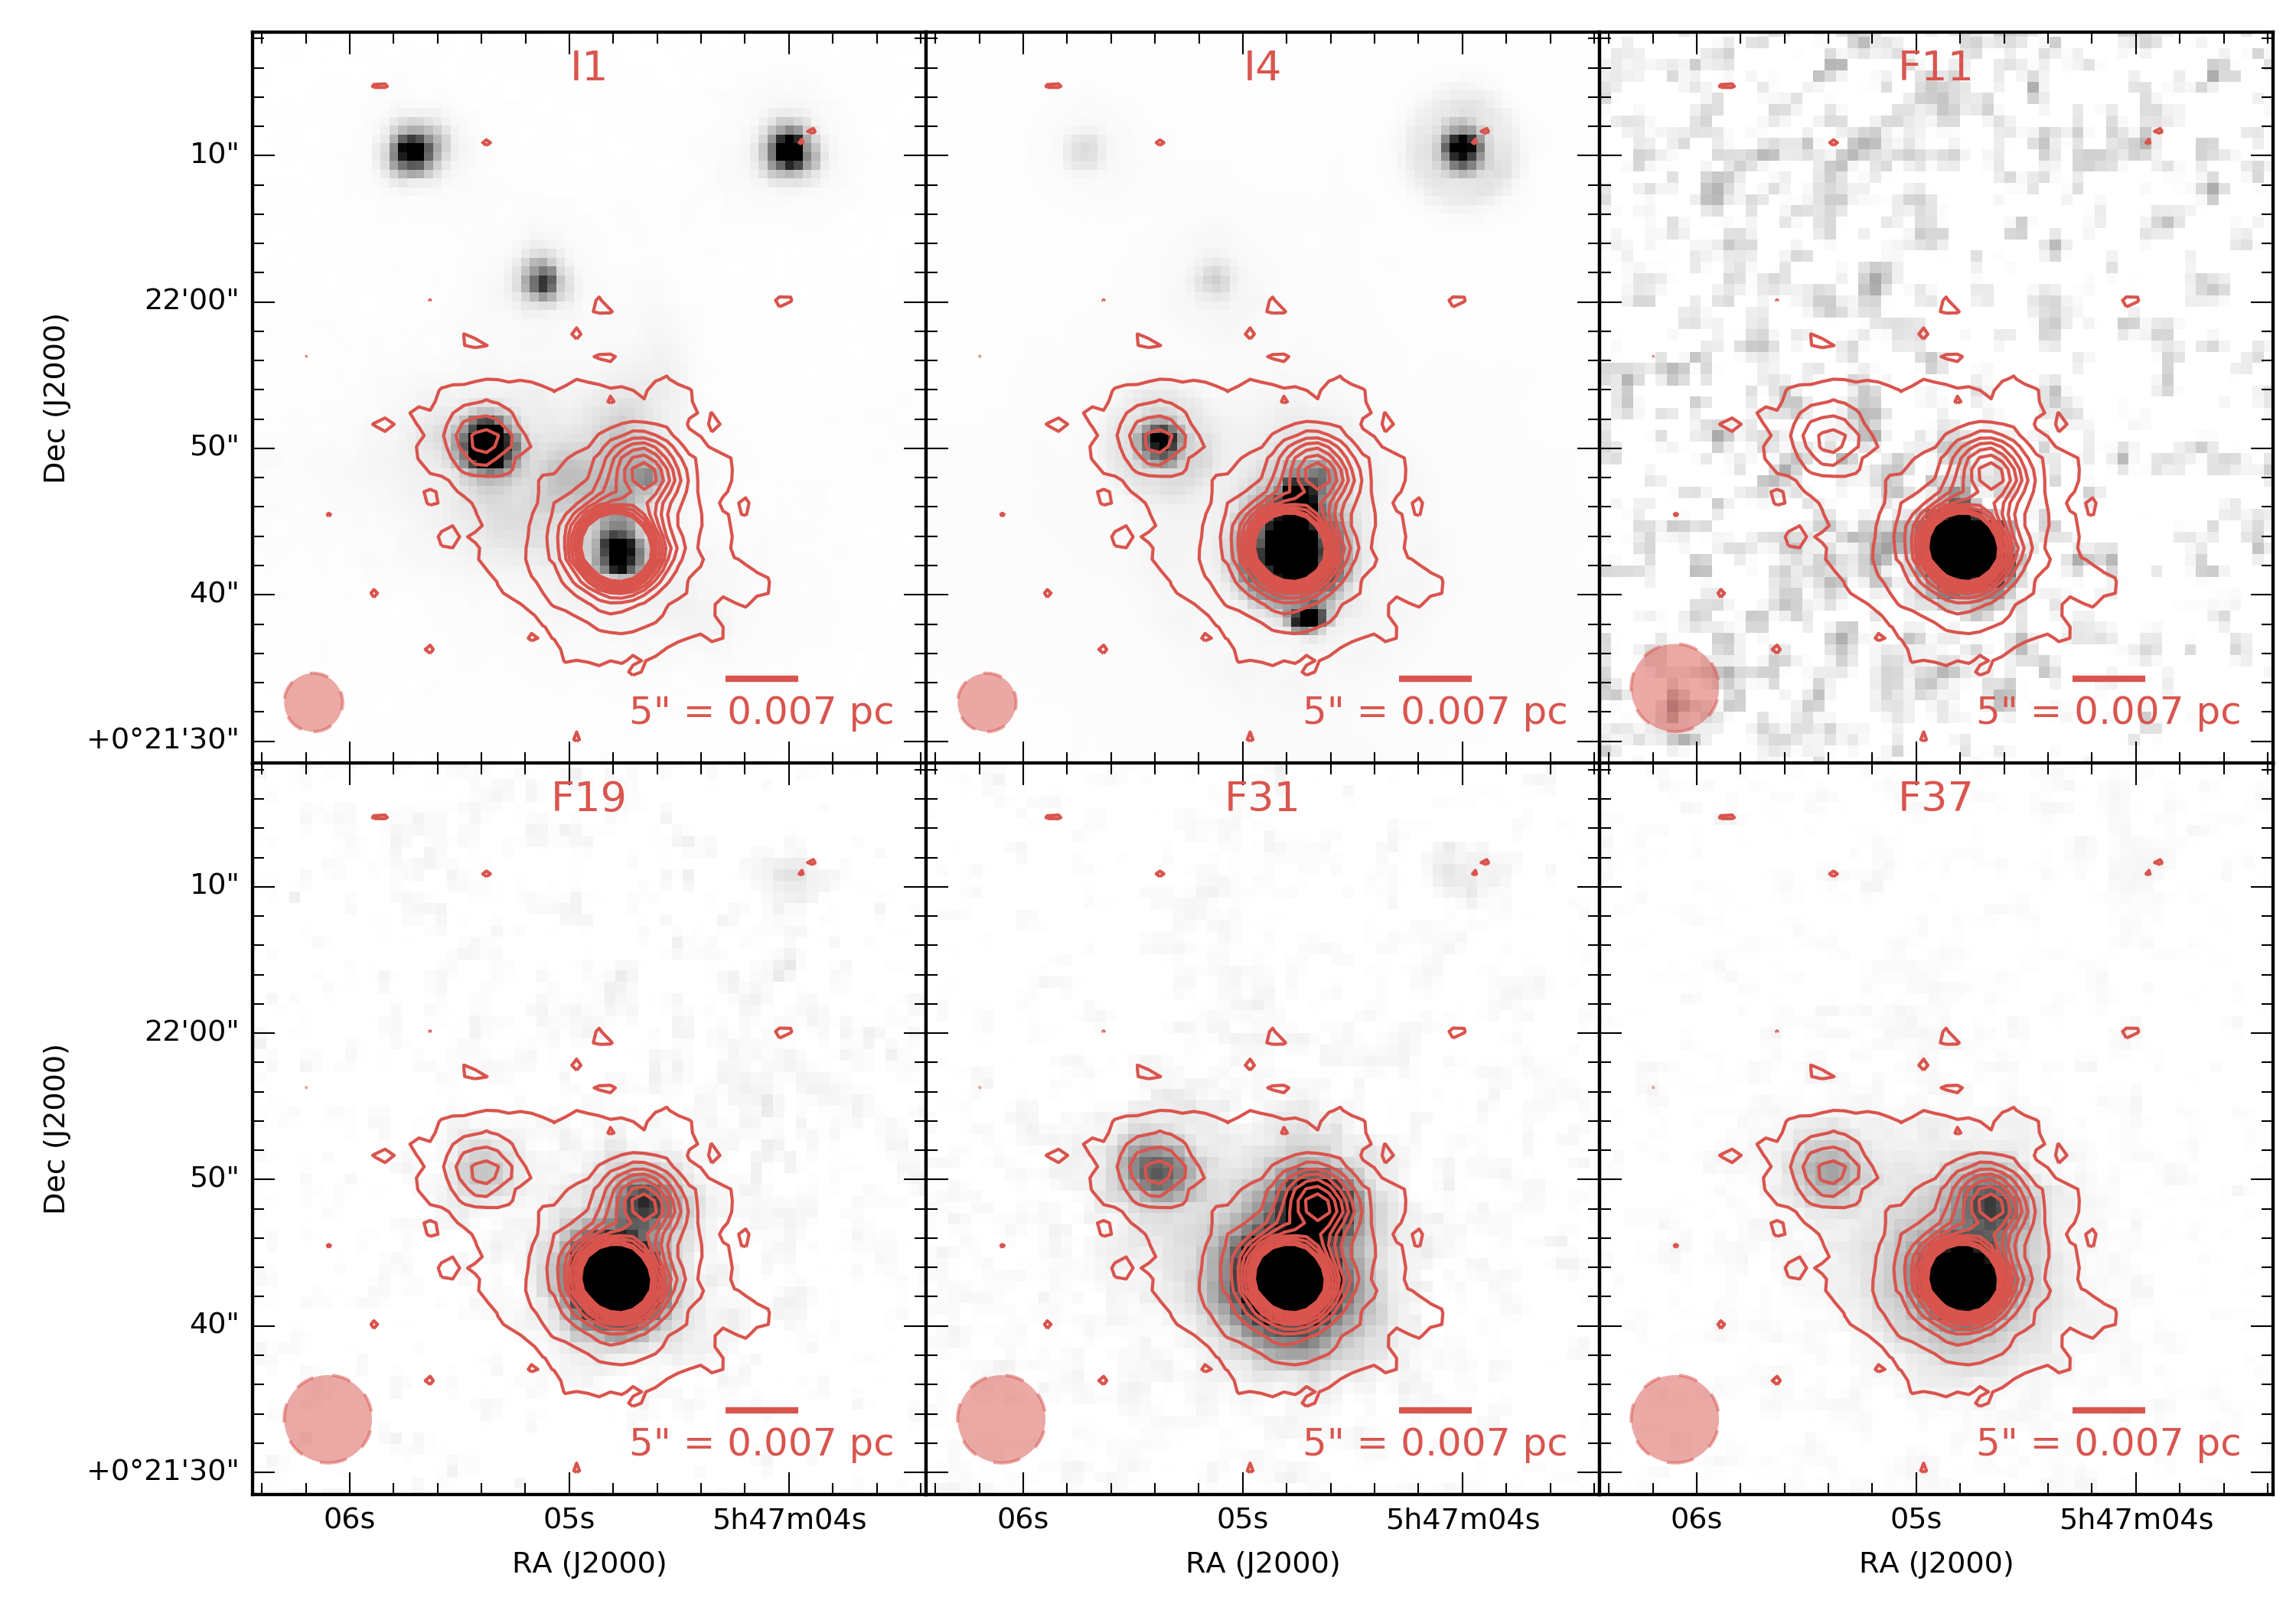
\includegraphics[width=1\textwidth]{Figures/NGC2071_mosaic.png}
%\label{fig:NGC2071_mosaic}
%\caption{The core of IRAS20050+2720 is seen in the four bands of the \textit{Spitzer} IRAS instrument, as well as with the four FORCAST bands. The increased resolution of FORCAST compared to previous instruments allows to match the long-wavelength emission with its short wavelength counterpart. The stretch in each image is adjusted for optimal readability. The white contours correspond to the FORCAST \SI{37}{\micro\meter} emission [mention the contour levels]. The red circles indicate the location of the five FORCAST point sources in the core.}
%\end{center}
%\end{figure}
%
%\begin{figure}
%\begin{center}
%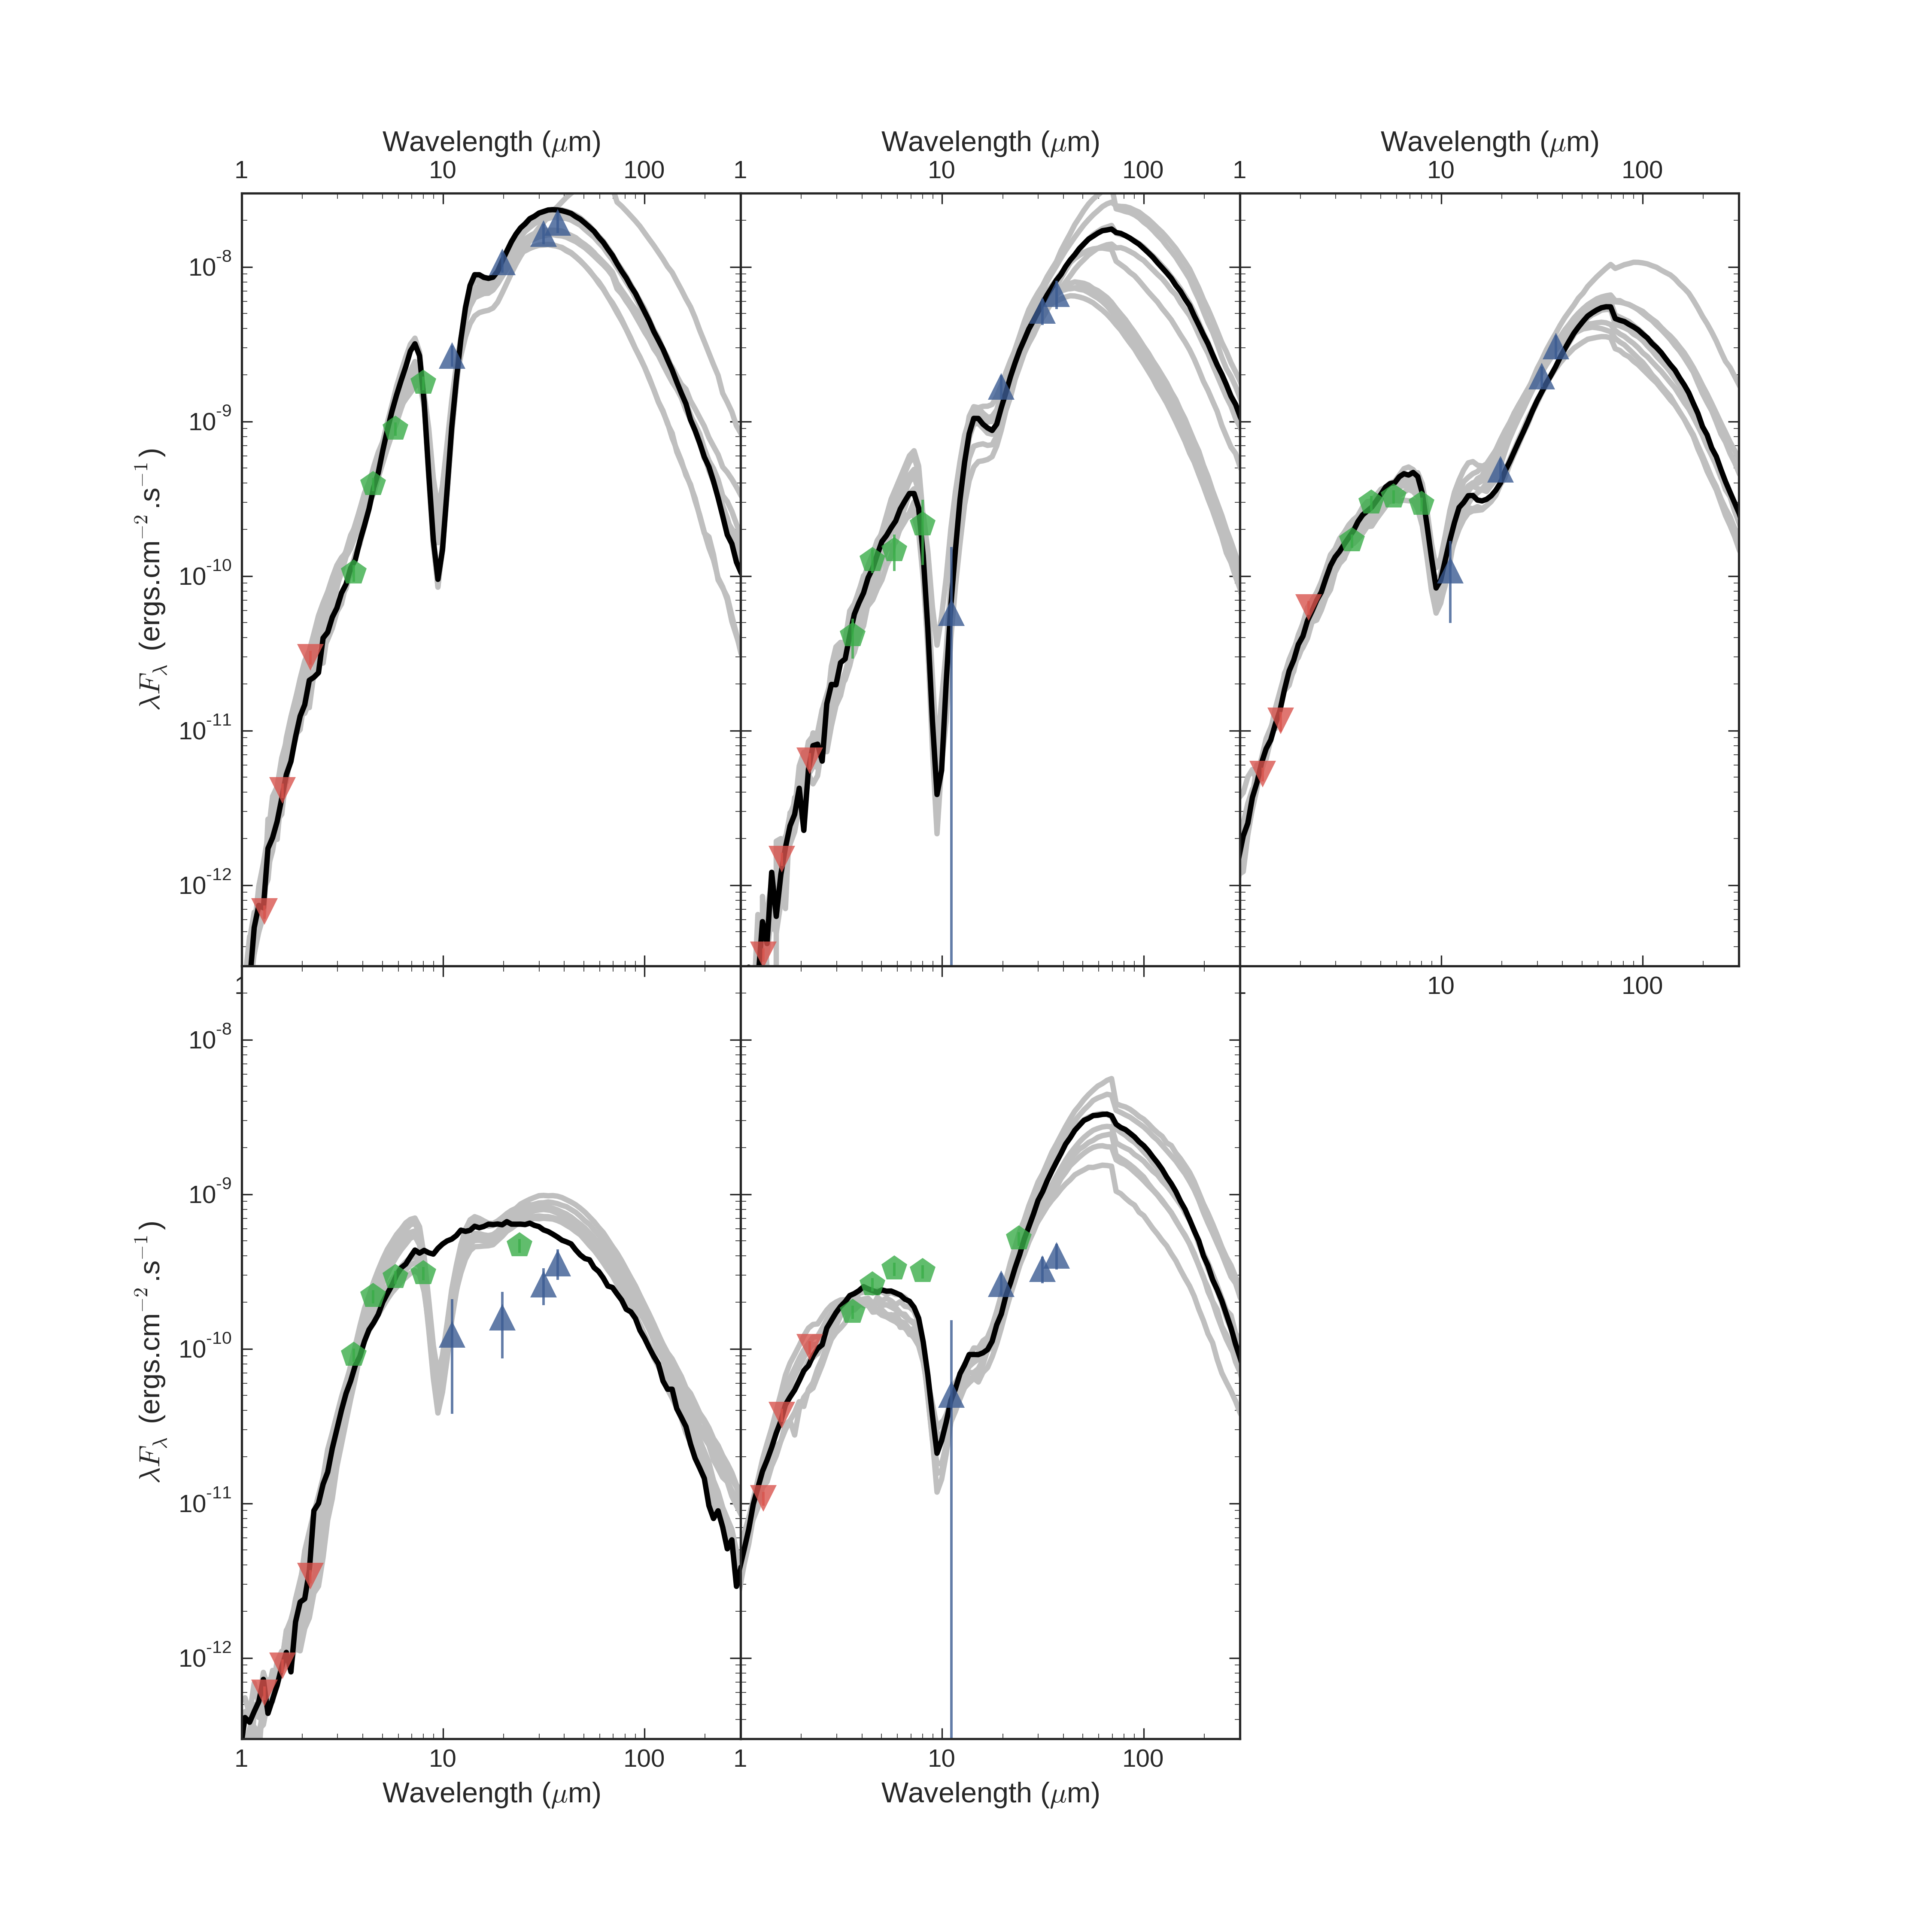
\includegraphics[width=1\textwidth]{Figures/NGC2071_SEDs.png}
%\label{fig:NGC2071_SEDs}
%\caption{}
%\end{center}
%\end{figure}
%
%\subsubsection{SEDs}
%
%\subsubsection{Upper limits on other sources in the field}
%
%
%\subsection{Summary}
%
%Put here the table of photometry + flags
%
%
%
%\section{SED and dust modeling}
%
%YE05 assumed the dust opacities of Ossenkopf \& Henning
%(1994) appropriate for thin ice mantles after 105 year of coagulation at a gas density of 106 cm-3 (OH5 dust), which several recent studies have shown to be appropriate for cold, dense cores (e.g., Evans et al. 2001; Shirley et al. 2002; Young et al. 2003; Shirley et al. 2005) [LOOK AT REST OF DISCUSSION IN DUNHAM et al. 2010]
%
%\subsection{Radiative transfer models}
%
%We use radiative transfer models to fit the SEDs we observe and extract physical parameters. We explored the tool by \cite{Robitaille:2006cb} as a starting point for this process. While the tool provides results that fit the data well, the large number of parameters makes it difficult to draw meaningful conclusions on the real physics behind the observations. We have observed a large amount of cross-correlations between the model parameters, as well as many local minimas in the $\chi^2$ minimization scheme that is used.
%
%In an effort to understand the dependence of the observations with the physical parameters used in the models, we use the HYPERION radiative transfer code \citep{Robitaille:2011fc} and create our own grid of models by varying a small amount of meaningful parameters. HYPERION is a very versatile code with lots of options for various geometries, but we simplify the problem to its most essential components: a circularly symmetric disk with a power-law envelope.
%
%We explore the various geometries and parameters that are available in the code, and come to following conclusions:
%\begin{enumerate}
%\item Modeling accretion through an $\alpha$-disk instead of a flared disk is equivalent to increasing the central luminosity by an appropriate amount. Hence, we use only standard flared disks and quote a total central luminosity
%\item It is good enough to only vary the total luminosity of the central object, instead of varying its mass, radius and temperature
%\item Models are very insensitive to disk mass, when the envelope's mass is larger
%\item The model is sensitive to the envelope's mass distribution within a given radius, but not sensitive to the envelope's inner or outer radius
%\item The outer radius of the disk has no effect on the models
%\item The inner radius of the envelope 
%\end{enumerate}
%
%Based on our exploration of HYPERION, we proceed with the following simulation set up. We use a density structure composed of a standard flared disk of \SI{e-3}{\Msun} that extends from the dust sublimation radius out to 50~AU. The scale height at the dust sublimation radius is set to be 10\% of that radius. The disk's flaring power is a constant set to $\beta=1.1$. 
%
%We add an envelope with a central cavity. The envelope extends from 30~AU out to a variable radius, and has a variable mass and power law exponent. The inner cavity has a constant 25 degree opening angle. Setting this latter parameter has some effect that is correlated with the viewing angle.
%
%All elements in our model are using the same dust model by \cite{Draine:2003di}. We have experimented with various other types of dust models, notably with the OH5 dust [REFERENCE], as it was suggested in [CITE TRACY]. We found that the fits with the OH5 dust were much worse. In most cases, it was particularly difficult to fit the \SI{10}{\micro\meter} silicate absorption feature. 
%
%We use a variable foreground extinction also with the same dust model, as we anticipate that most of the extinction along the line of sight will occur in the cluster itself. We chose to not use any ambient medium, as they complicated the interpretation of the results.
%
%We run our simulations using $10^5$ photons, and spherical grids with 199 radial cells, 49 meridional cells, and 1 single azimuthal cell. We have tested these various parameters and sought an optimum of fast computing times and low statistical noise. With this, the calculated uncertainties are a few percent at long wavelengths and can be on the order of 10 to 15 percent at short wavelengths. This is acceptable since the short wavelength range is largely used in the fit to determine the overall external extinction magnitude. At the wavelenghts relevant for the IRAC fluxes, the uncertainties due to the simulation are on the order of 5\% - less than our estimated measurement error. With these parameters, a typical model takes about 5-10 minutes to run on a standard desktop computer. Our wrapper software allows us to run multiple different grids in a row and merge them into one single entity that we can feed to a minimization routine.
%
%In order to fit the data, we use the $\chi^2$ method described in \cite{Robitaille:2007dl}, with the exception of the overall optimal scaling step. We calculate the $\chi^2$ for our targets with all calculated models, inclinations, and a range of values of foreground extinction magnitudes.
%
%
%%Table of set parameters]
%
%%variable parameters: envelope mass, envelope density power law, source luminosity, inclination, extinction
%
%
%
%
%%This section discusses how we set up a grid of models to fit, and why we moved away from Robitaille's sedfitter. Maybe show some results from the Robitaille's fits?
%
%\subsection{Extracting physical parameters from the fits}
%This section discusses the results from the fits: best fits, parameter estimation and variation about the best fits, color-color diagrams, etc.
%\begin{itemize}
%\item \citep{Shirley:2000gh}: typical masses of protostars are a few tenths to \SI{2}{\Msun}. 
%
%\end{itemize}
%
%
%\section{Discussion}
%
%\section{Conclusion}
%blabla
